\chapter{Исследования собственных движений быстрых звезд в Пулковcкой обсерватории. Адаптация метода Вилена} \label{ch:ch3}
\section{Наблюдения быстрых звезд в Пулковской обсерватории. Вычисление новых собственных движений с использованием положений звезд из различных различных каталогов} \label{sec:ch3/sect1}
Как уже упоминалось, в ЛАЗА ГАО РАН  реализуется программа астрометрических исследований близких карликов, в том числе и с привлечением оригинальных пулковских наблюдений. Основная часть наблюдений выполнена с помощью Нормального астрографа ($D=330$~мм, $F=3467$~мм).  Кроме того, используется  26$''$--рефрактор ($D=650$~мм, $F=10\,413$~мм), благодаря относительно большому фокусному расстоянию которого удалось выполнить наблюдения с целью определения тригонометрических параллаксов звезд \cite{2010AstL...36..576K}, \cite{2013MNRAS.435.1083K}. Часть наблюдений проводится на метровом зеркальном телескопе <<Сатурн>> \cite{2015arXiv151101642K}, который после восстановления активно используется для наблюдений тел Солнечной системы и быстрых карликов.

В 2011 году была опубликована работа \cite{2011AstL...37..420K}, посвященная исследованию собственных движений быстрых звезд низкой светимости. Это можно назвать первым этапом апробации метода Вилена с применением пулковских наблюдений. Для данного исследования были взяты наблюдения быстрых ($\mu>300 mas/yr$ по данным каталога LSPM \cite{2005AJ....129.1483L}, \cite{2008IAUS..248...74L}) звезд, проводимых с 2006 года на Нормальном астрографе Пулковской обсерватории в зоне склонения $+30^{\circ}$~--~$+70^{\circ}$. В результате обработки около 10\,000 кадров 1123 включенных в программу наблюдения звезд были получены положения 414 объектов. Для аппроксимации звездных изображений использовался профиль Лоренца, параметры функции рассеивания точки (PSF) рассчитывались в кольце радиусом 20~пикселей. Астрометрическая редукция проводилась в два этапа, при этом использовался метод шести постоянных в системе  HCRF/UCAC3. UCAC3 \cite{2010AJ....139.2184Z} в качестве опорного был выбран в связи с него высокой плотностью распределения звезд по небесной сфере. Однако стоит отметить, что при работе с данным каталогом пришлось проявить некоторую осторожность из-за больших систематических ошибок собственных движений звезд северного полушария, что было отмечено авторами  каталога PPMXL \cite{2010AJ....139.2440R}. В ходе первого этапа редукции были вычислены ошибки на основе остаточных разностей пиксельных координат и проведен анализ на уравнение блеска, что было учтено на втором этапе редукции. В итоге ошибки единицы веса по обеим координатам в среднем составили 70~mas. Однако, стандартные ошибки средних положений звезд по нескольким кадрам оказались в основном в рамках 10~--~20~mas. Распределение стандартных ошибок определения экваториальных координат представлено на рисунке~\ref{fig:11erpos}

\begin{figure}[pt]
 \centering
 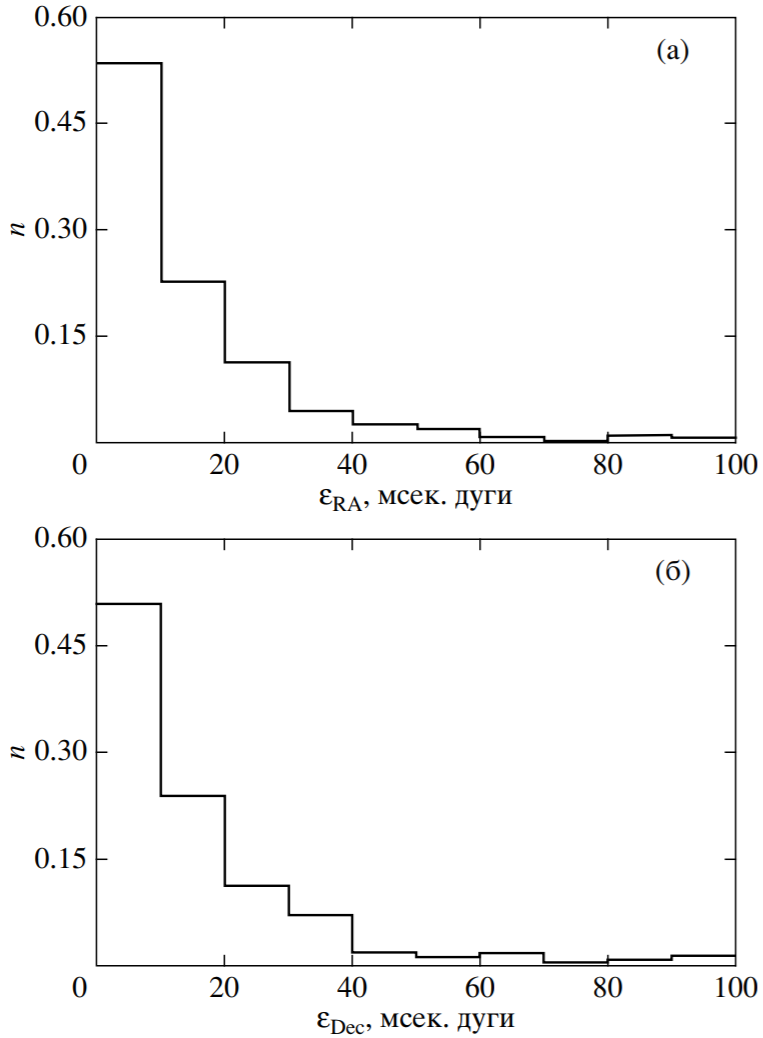
\includegraphics [scale=0.75] {khrutskaya3}
 \caption{Распределение стандартных ошибок определения экваториальных координат быстрых звезд, полученных в рамках работы \cite{2011AstL...37..420K}. Взято из указанной работы, рис. 3.}
 \label{fig:11erpos}
\end{figure}

Для расчета собственных движений помимо оригинальных положений были использованы координаты звезд из различных обзоров, в том числе CMC14, M2000, 2MASS, а также актуальный на тот момент SDSS DR7. Средние эпохи наблюдений этих каталогов лежат в пределах 1997~--~2004~г., стандартные ошибки в среднем составляют 40~--~80~mas. Координаты звезд в использованных каталогах формально отнесены к системам HCRF/UCAC2 или HCRF/Tycho--2, которые на приемлемом уровне точности можно соотносить с системой HCRF/UCAC3. Разности эпох для расчета собственных движений составили 6~--~13~лет, а средняя точность получившихся собственных движений оказалась в пределах 1~--~10~mas/yr (см. рисунок~\ref{fig:11ermu}).

\begin{figure}[pt]
 \centering
 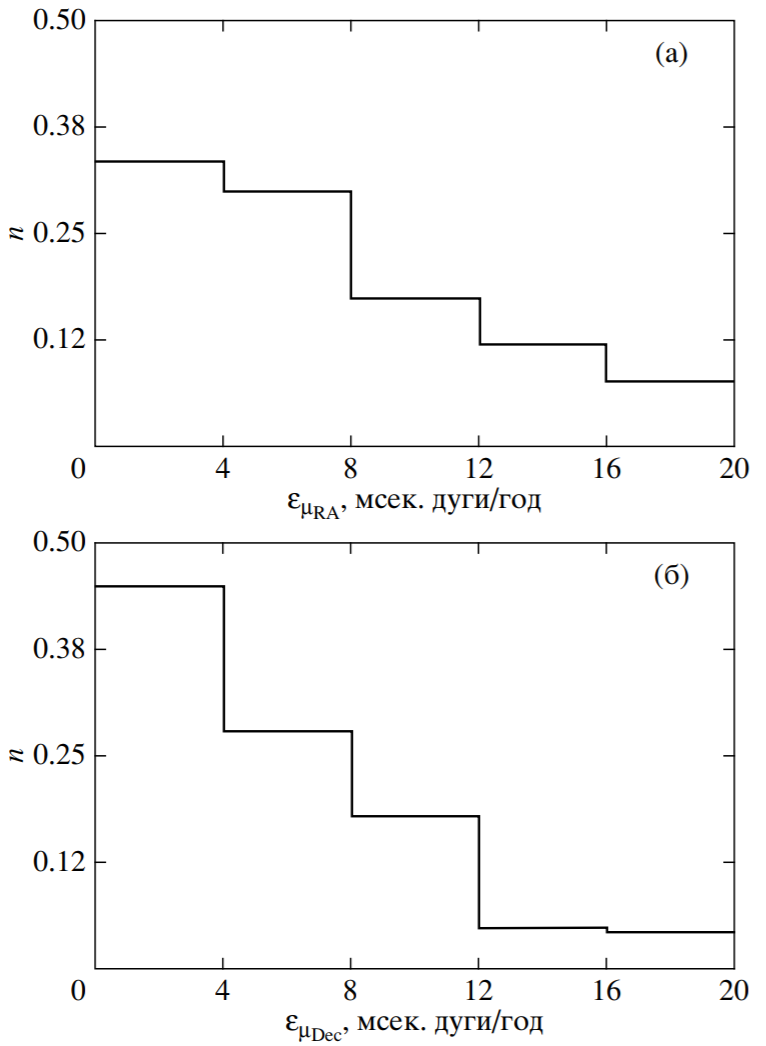
\includegraphics [scale=0.75] {khrutskaya4}
 \caption{Распределение стандартных ошибок определения собственных движений быстрых звезд, полученных в рамках работы  \cite{2011AstL...37..420K}. Взято из указанной работы, рис. 4.}
 \label{fig:11ermu}
\end{figure}

Далее для исследуемых звезд по аналогии с методом, описанном в главе 1., сравнивалась значимость по отношению к ошибкам определения разности полученных собственных движений и движений каталога LSPM, рассчитанной на временной базе около 50 лет. В данном случае полученные собственные движения можно считать квазимгновенными, а взятые из каталога LSPM "--- квазисредними. Значимость таких разностей (\glqq космических ошибок\grqq\  в терминологии Р. Вилена) была оценена через параметр F:
\begin{equation}
\label{eq:KhrF}
F^2=\frac{\Delta\mu^2_{RA}}{\epsilon^2_{\mu_{RA}}}+
\frac{\Delta\mu^2_{Dec}}{\epsilon^2_{\mu_{Dec}}}
\end{equation}
где $\Delta\mu_{RA}$ и $\Delta\mu_{Dec}$ "--- разности компонент квазисредних и квазимгновенных собственных движений звезды, а $\epsilon_{\mu_{RA}}$ и $\epsilon_{\mu_{Dec}}$ "--- соответствующие среднеквадратические ошибки. Кандидатом в $\Delta\mu$--двойную с вероятностью 95\% считалась звезда при $F>2.59$. Таких звезд оказалось 70 из выборки. В качестве проверки в работе было отмечено, что среди исследованных оказалось 42 звезды из каталога WDS \cite{2001AJ....122.3466M}, у 15 из которых были обнаружены значительные величины параметра F.
\section{Вычисление собственных движений на основе прямой редукции пиксельных координат} \label{sec:ch3/sect2}
Необходимо обратить внимание, что в работе, описанной в предыдущем разделе, имеют место некоторые недостатки. Во-первых, стоит отметить, что положения звезд в использованных каталогах лишь формально относятся к единой системе, неизвестные взаимные систематические ошибки могли оказать серьезное влияние на конечный результат. Кроме того, использовать F--статистику напрямую из работы Вилена было отчасти неправомерно. Ведь в оригинальной работе Вилена рассматривались ярчайшие звезды каталога HIPPARCOS и их высокоточные собственные движения, полученные в течение периода около 3 лет. Это гарантировало \glqq гауссовость\grqq\  распределения ошибок.

В качестве логичного продолжения предыдущей работы, было принято решение провести исследования собственных движений быстрых звезд, рассчитанных методом прямой редукции пиксельных координат с кадра на кадр, а также более тщательно оценить предельные величины параметра F, учитывая исследуемый материал.
\subsection{Формирование списка звезд и особенности наблюдений} \label{subsec:ch3/sect2/sub1}
Как и в предыдущей работе \cite{2011AstL...37..420K}, в программу наблюдений были включены звезды каталога LSPM. В основной список вошли 1972 звезды до $17^m$ в зоне склонений от $30^{\circ}$ до $70^{\circ}$. В основном это звезды c $\mu>300$~mas/год (1507 звезд). По разным причинам были добавлены 465 звезд. Некоторые из них имеют большое значение фотометрического параллакса, ряд звезд был добавлен для анализа возможности исследований сравнительно медленно двигающихся объектов ($\mu>100$~mas/год).

Распределение звезд наблюдательной программы по небесной сфере показано на рисунке~\ref{fig:15alloc}. Рисунок~\ref{fig:15hist} демонстрирует как программные объекты распределены по величине полного собственного движения, по блеску, по массам и расстояниям от Солнца. В целом, это почти полная выборка. Каталог LSPM содержит почти все существующие быстрые звезды до $19^m$ (Лепин и Шара, 2005 ). Поэтому можно сказать, что в пулковскую наблюдательную программу вошли все звезды, которые только можно эффективно наблюдать в Пулкове в соответствующих диапазонах по блеску и величине собственного движения.

\begin{figure}[h]
\centering
%\includegraphics [scale=1] {fig_1.ps}
\includegraphics[width=0.49\columnwidth]{fig1_a.eps}
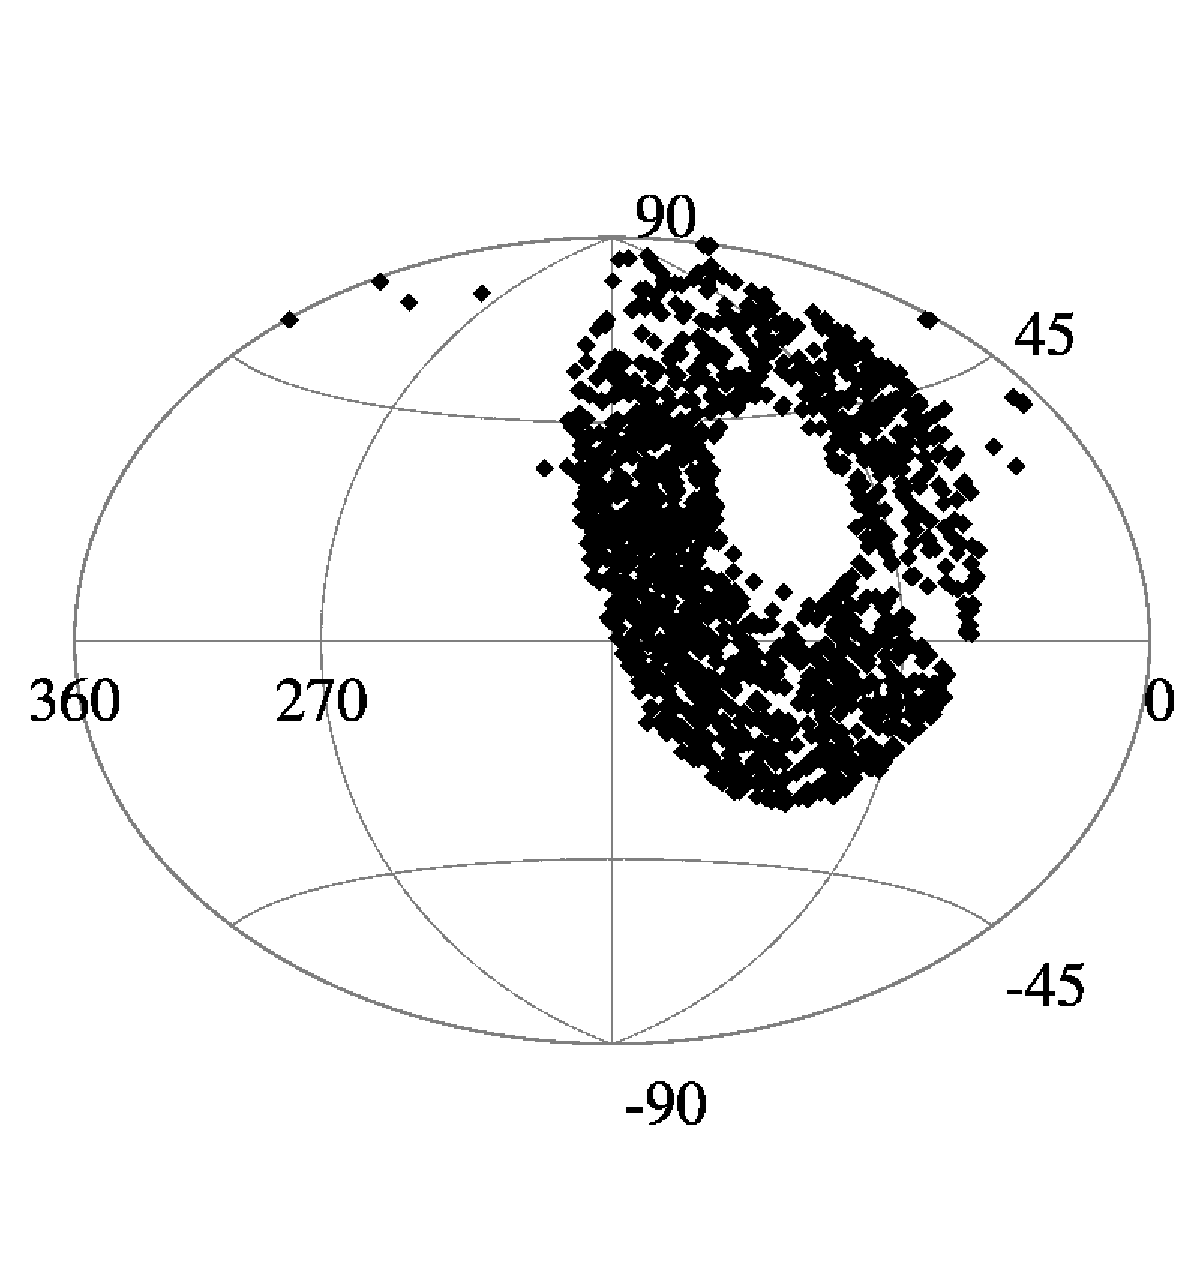
\includegraphics[width=0.49\columnwidth]{fig1_b.eps}
\caption{Распределение звезд пулковской программы по небесной сфере в экваториальной (слева) и галактической (справа) системах координат. Взято из работы \cite{2015AstL...41..833K}, рис.1.}
 \label{fig:15alloc}
\end{figure}

\begin{figure}[h]
\centering
% \includegraphics [scale=1] {fig2.ps}
\includegraphics[width=0.53\columnwidth]{fig2a.eps}
\includegraphics[width=0.46\columnwidth]{fig2b.eps}
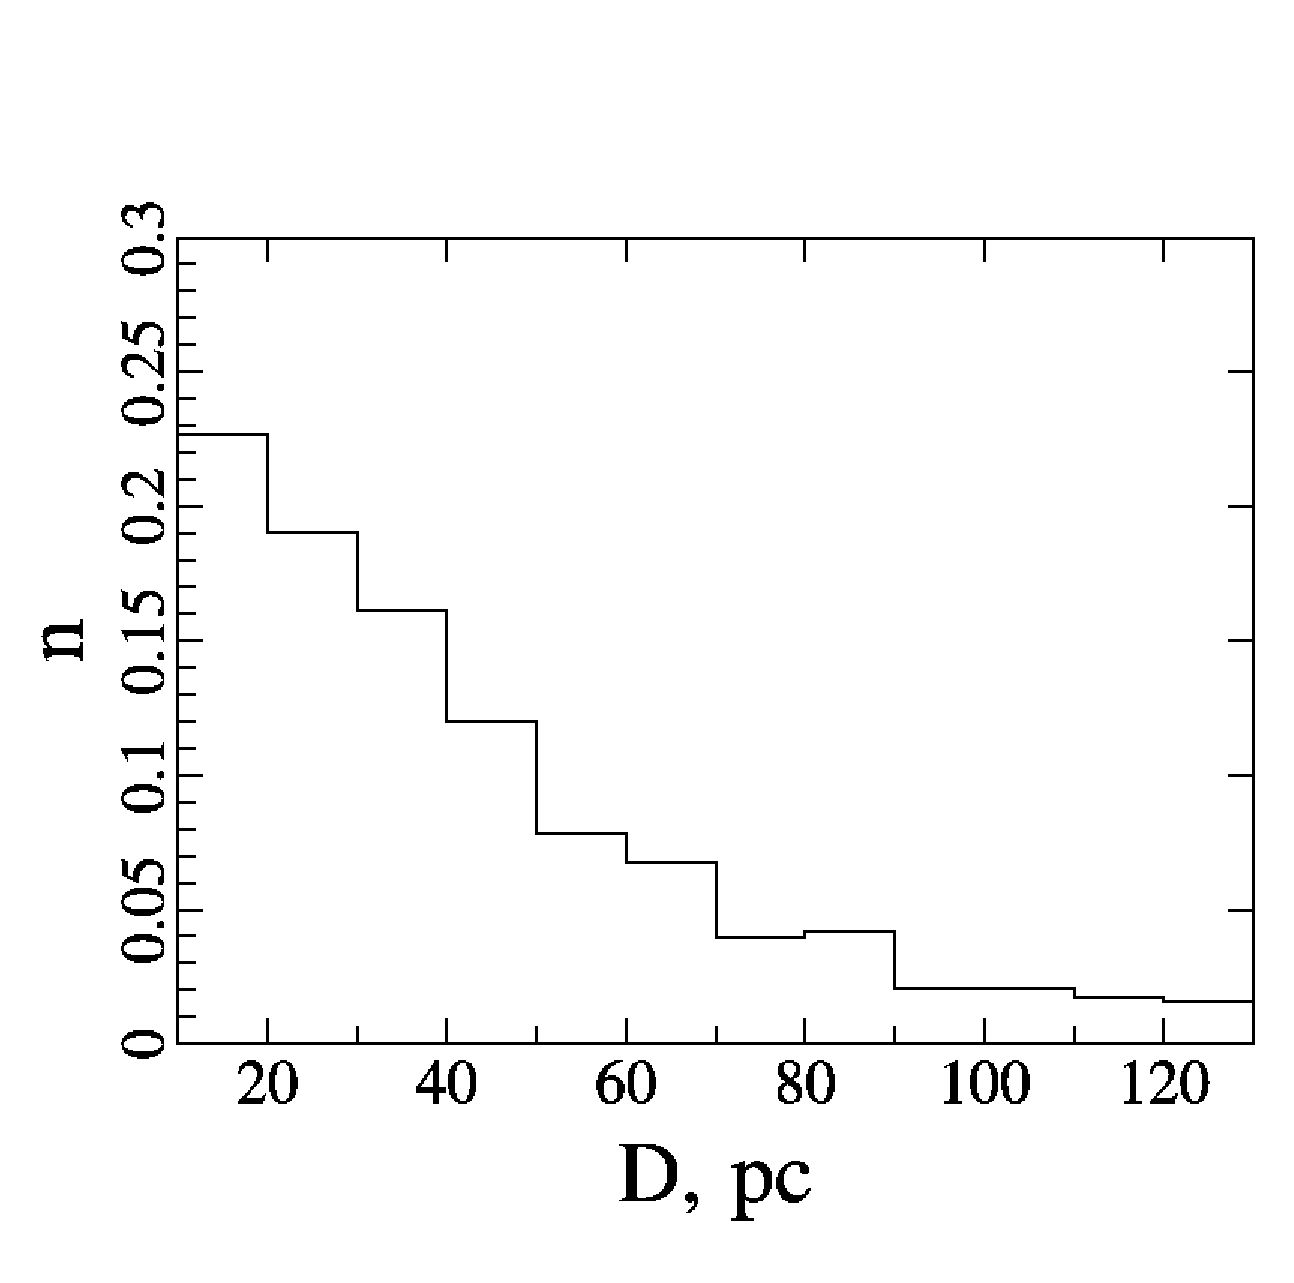
\includegraphics[width=0.49\columnwidth]{fig2c.eps}
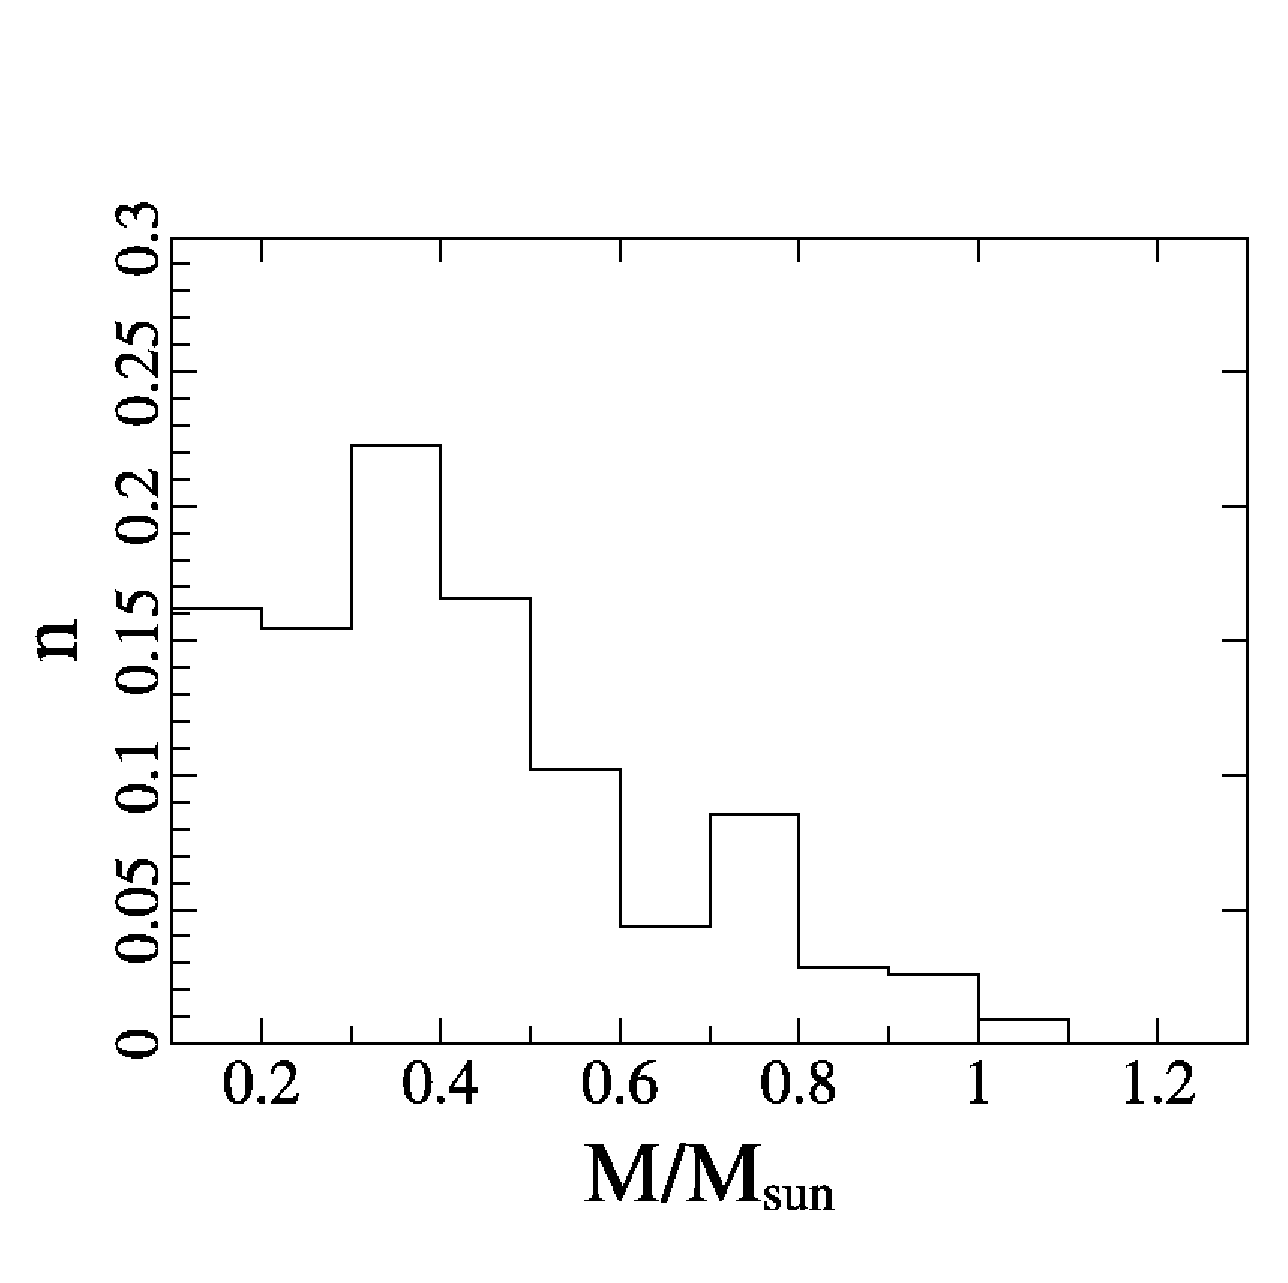
\includegraphics[width=0.49\columnwidth]{fig2d.eps}
\caption{Распределение звезд пулковской программы по величине полного собственного движения (сверху и слева), по звездной величине (сверху и справа), по расстоянию от Солнца (снизу и слева) и по массе (справа и внизу). Взято из работы \cite{2015AstL...41..833K}, рис.2.}
\label{fig:15hist}
\end{figure}

ПЗС-наблюдения также велись с помощью Нормального астрографа Пулковской обсерватории (D = 330~мм, F = 3500~мм) с 2008 по 2015 годы. Они были необходимы чтобы повысить точность определения квазимгновенных собственных движений звезд.  До 2014 года использовалась камера S2C (рабочее поле "--- $18\times16$~arcmin при масштабе 900~mas/pix). В 2014 и 2015 годах была установлена камера \mbox{SBIG ST-L-11K} (рабочее поле - $35\times23$~arcmin, масштаб - 530~mas/pix). Съемка проводилась при часовых углах $\pm1^h$ сериями от 5 до 10 кадров с экспозициями 60 или 120 секунд в зависимости от блеска исследуемой звезды. В ряде случаев для слабых звезд число кадров в серии увеличивалось до 40, чтобы достичь нужной величины соотношения сигнал/шум путем суммирования отдельных кадров.
\subsection{Использование данных цифровых обзоров неба} \label{subsec:ch3/sect2/sub2}
Уже давно в астрономическую практику вошло понятие \glqq виртуальной обсерватории\grqq , когда результаты наблюдений (в том числе и изображения участков неба) доступны с помощью сети Интернет.  Для нашей задачи представляли интерес обзоры неба, содержащие ПЗС-кадры или сканы фотографических пластинок для всего неба или для значительной его части. В данной работе использованы данные обзоров SDSS~DR12\footnote{\textit{http://dr12.sdss3.org/fields/}} \cite{2015ApJS..219...12A}, 2MASS\footnote{\textit{http://irsa.ipac.caltech.edu/ibe/}} \cite{2003tmc..book.....C}, WISE\footnote{\textit{http://irsa.ipac.caltech.edu/applications/wise/}} \cite{2010AJ....140.1868W} и STScI DSS\footnote{\textit{http://archive.stsci.edu/cgi-bin/dss\_form}} \cite{1998asal.confE...3L} (сканы пластинок Паломарского обзора неба POSSI-O и POSSII-J).

Для всех перечисленных обзоров существует удобный интерфейс, обеспечивающий возможность запроса fits--файлов. Загрузка необходимых данных осуществлялась автоматически с помощью специально созданного приложения и заняла несколько дней из-за большого объема данных обзора WISE (поля в этом обзоре сняты с многочисленными перекрытиями). Для обзора WISE использовались кадры только \glqq холодной\grqq\  части миссии в полосах W1 и W2, чтобы гарантировать приемлемое значение отношения сигнала к шуму для изображений слабых звезд.

\subsection{Определение пиксельных координат} \label{subsec:ch3/sect2/sub3}
Все ПЗС-кадры и сканы пластинок POSS1 и POSS2 анализировались по единой схеме. Для аппроксимации звездных изображений на каждом кадре использовалось shapеlet--разложение \cite{2005MNRAS.363..197M}, описанное в предыдущей главе.

Пиксельные координаты фотоцентра звездного изображения варьировались по схеме, приведенной в цитированной выше работе, чтобы гарантировать минимум суммы квадратов невязок. Этот же принцип применялся для автоматического подбора порядка разложения. Типичные примеры результатов аппроксимации изображений сравнительно яркой звезды на кадрах из разных обзоров приведены на рисунке~\ref{fig:15approx}. В целом, методика измерения изображений работает надежно. Некоторые проблемы наблюдались с выбором порядка разложения для кадров SDSS. Судя по структуре распределения невязок, можно предположить, что порядок несколько переоценен. Как показали результаты астрометрических редукций кадров обзора SDSS, это не критично для астрометрических измерений (для звезд c $V_{mag}$=14 сходимость пиксельных координат лежит в пределах 10~mas).

\begin{figure}[h]
\centering
 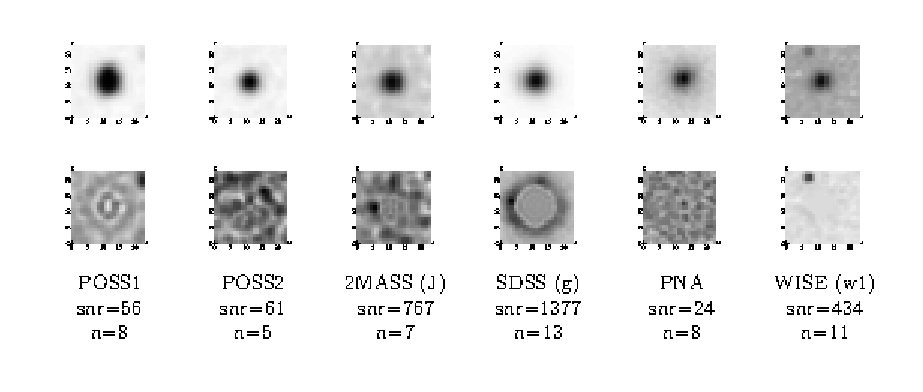
\includegraphics [scale=1.25] {fig3.eps}
\caption{Аппроксимация изображения звезды J0753+5106 ($V_{mag}$=14.2) на снимках различных обзоров неба. Верхний ряд содержит исходные изображения, нижний "--- результат вычитания \glqq реальное "--- модельное\grqq . Приведены отношение сигнал к шуму для пикселя с максимальным значением отсчета (snr) и порядок shapelet--разложения (n). Размер области изображения $24\times24$~pix. Взято из работы \cite{2015AstL...41..833K}, рис.3.}
\label{fig:15approx}
\end{figure}

\subsection{Анализ систематических ошибок координат звезд в разных обзорах} \label{subsec:ch3/sect2/sub4}
При построении астрометрических каталогов на основе ПЗС--наблюдений часто используется подход, базирующийся на формировании векторных полей остаточных разностей пиксельных координат звезд на основе всего массива данных. Для всех кадров данного обзора была произведена астрометрическая редукция. Постоянные кадра позволили вычислить остаточные разности пиксельных координат опорных звезд \glqq каталог "--- кадр\grqq .

Эти разности могут быть обусловлены комой, дисторсией и другими геометрическими искажениями. Они могут проявлять себя как зависимости невязок от координат и блеска. Примеры таких зависимостей показаны на рисунке~\ref{fig:15posL}. Исходя из приведенных графиков, с большой долей уверенности можно констатировать отсутствие уравнения блеска для пулковских ПЗС--кадров, заметную и сложную дисторсию для кадров космического обзора WISE. Для вычисления поправок рабочее поле кадра разделялось на квадратные (или прямоугольные) области, размеры которых подбирались так, чтобы туда попадало не менее 100 разностей в каждую группу по блеску (от $10^m$ до $16^m$ с шагом $1^m$).

\begin{figure}[h]
\centering
% \includegraphics [scale=1] {fig4.ps}
\includegraphics[width=0.7\columnwidth]{fig4a.eps}\\
\includegraphics[width=0.7\columnwidth]{fig4b.eps}
\caption{Примеры зависимостей остаточных разностей координат звезд от блеска и положения в кадре. Сверху "--- для пулковских ПЗС--кадров (масштаб "--- 0.950~arcsec/pix), снизу - для изображений WISE (в полосе W1, масштаб "--- 2.758~arcsec/pix). Взято из работы \cite{2015AstL...41..833K}, рис.4.}
\label{fig:15posL}
\end{figure}

В качестве поправок для геометрического центра области использовались средние величины от всех разностей, попавших в данную ячейку с соответствующими значениями координат центра и звездной величины. Величины поправок для любой точки и значения блеска вычислялись путем бикубической интерполяции. Примеры векторных полей остаточных разностей демонстрируются на рисунке~\ref{fig:15pixL}. Видно, что влияние значительной дисторсии телескопа WISE вполне можно выявить и корректно учесть. Кадры обзора SDSS свободны от значимых геометрических искажений. Уровень систематических ошибок составляет десятые и сотые доли пикселя (менее 40~--~50~mas).

\begin{figure}[h]
\centering
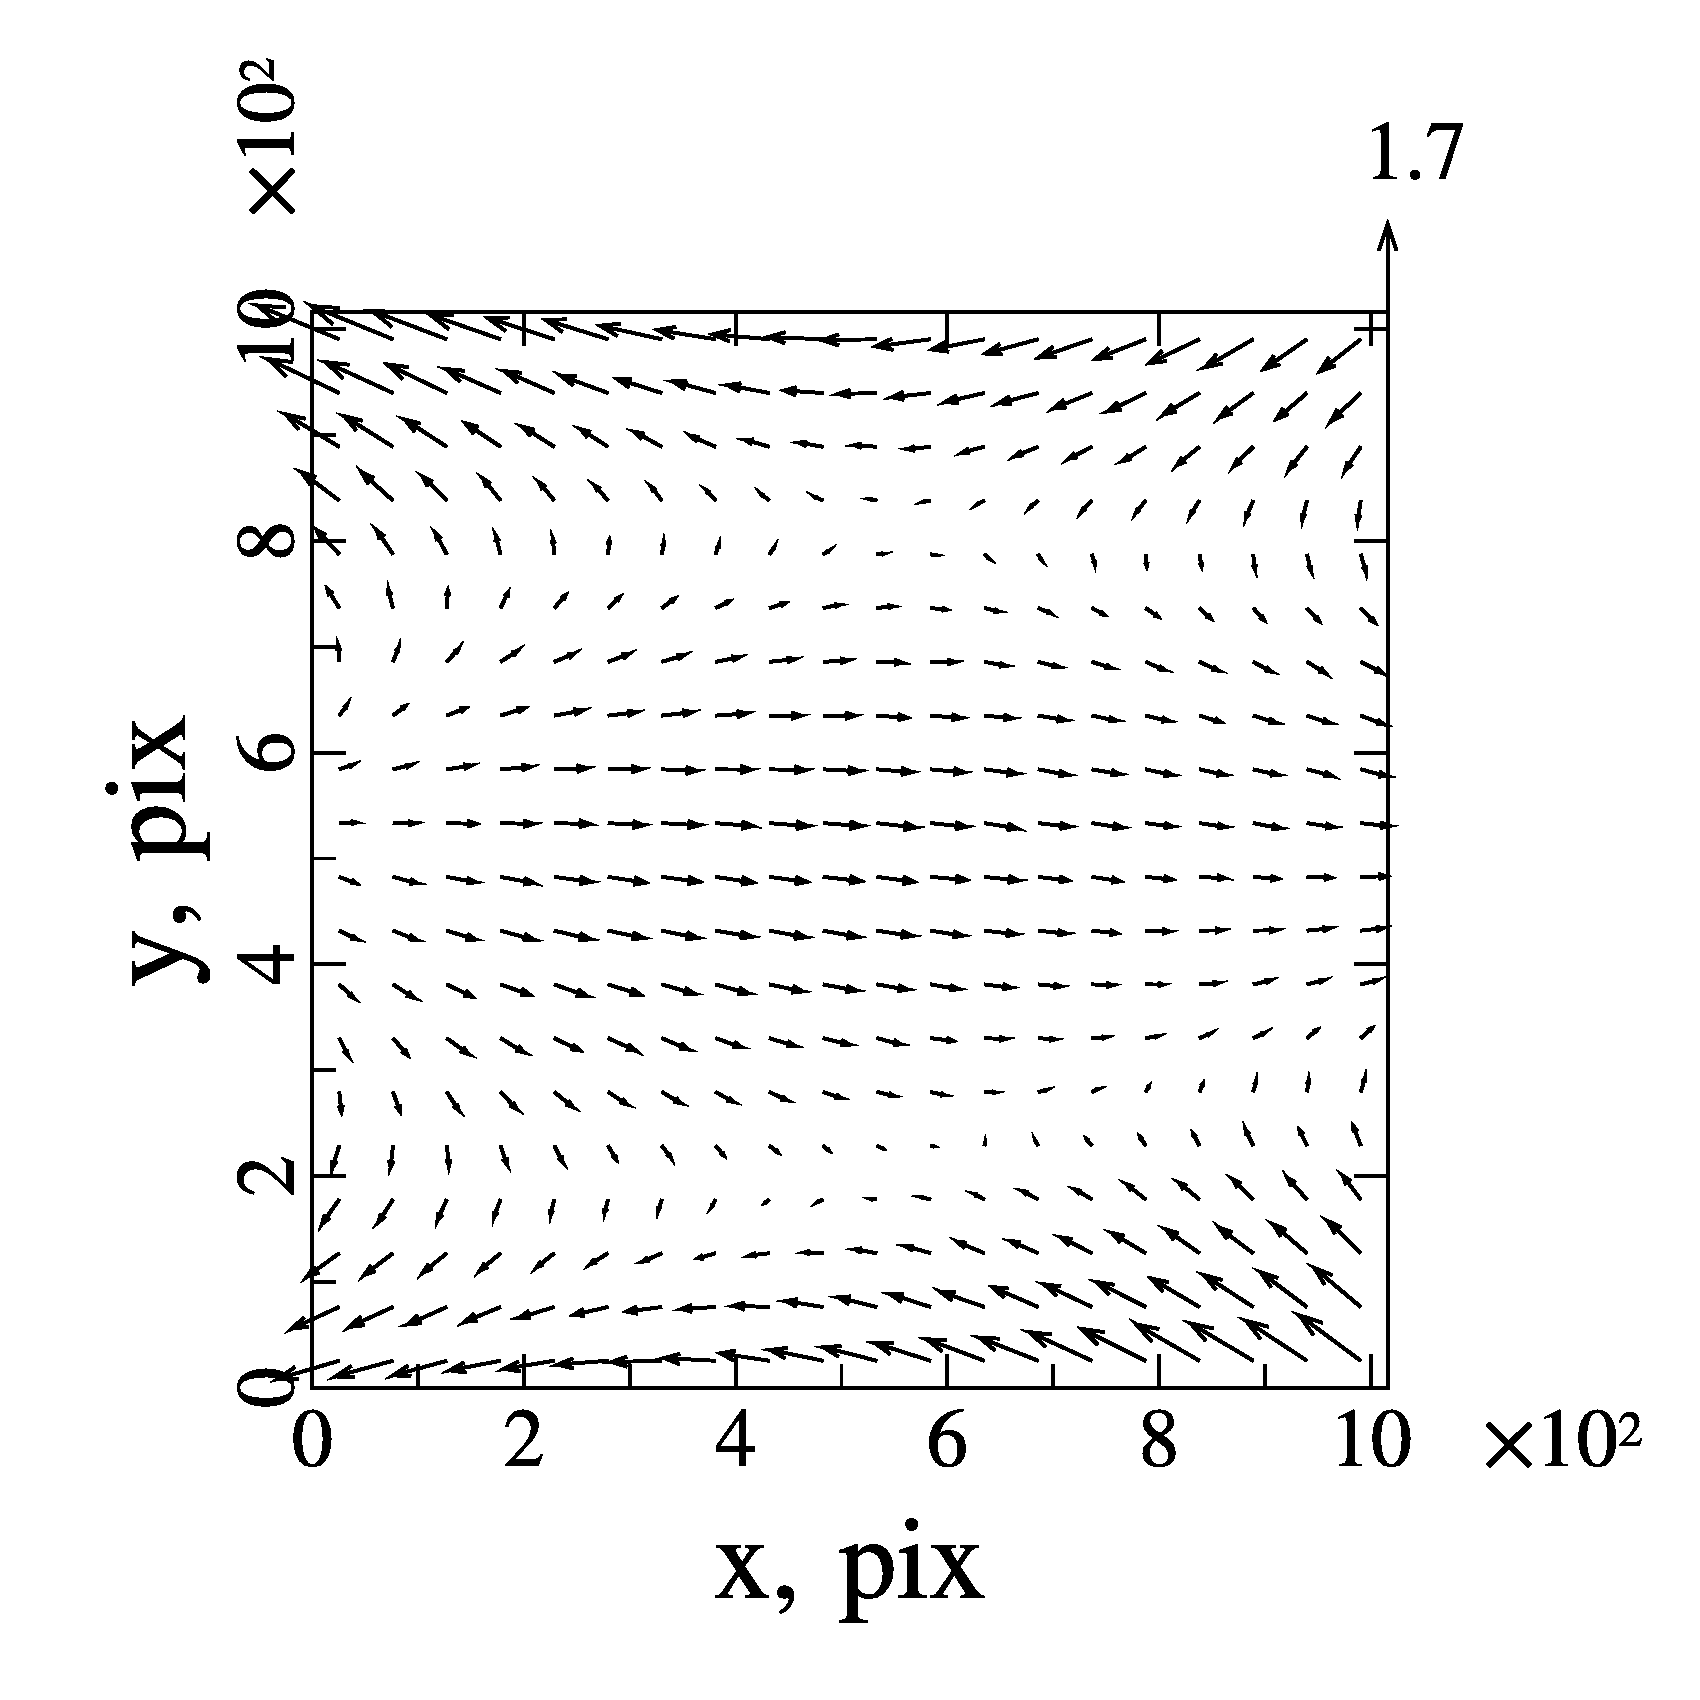
\includegraphics[width=0.49\columnwidth]{fig5a.eps}
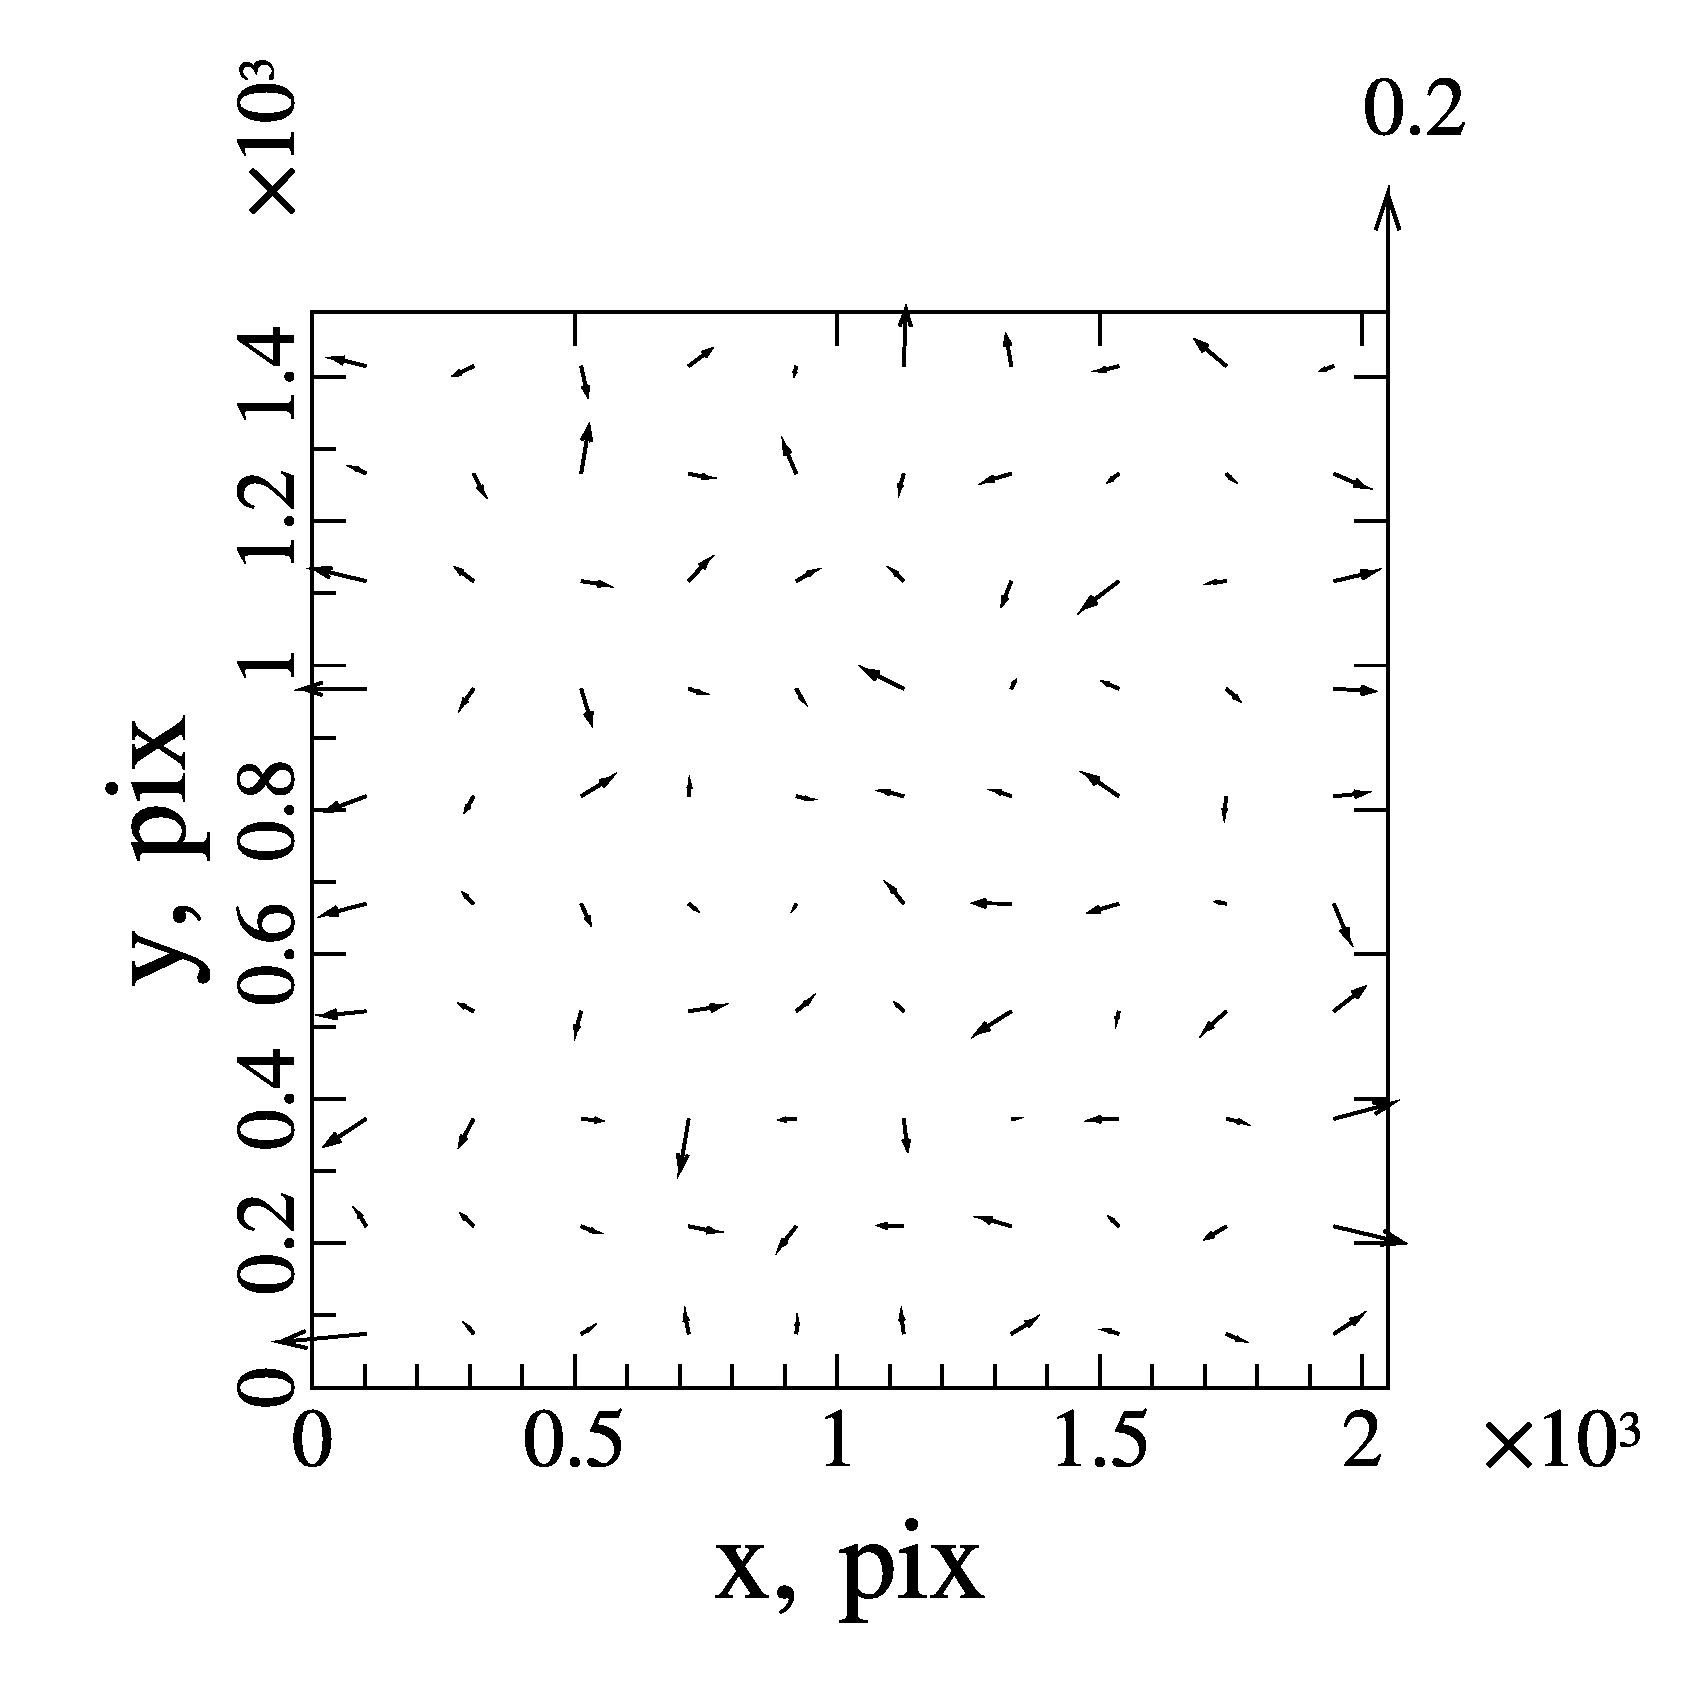
\includegraphics[width=0.49\columnwidth]{fig5b.eps}
\caption{Примеры векторных полей остаточных разностей пиксельных координат звезд в диапазоне $14^m$ -- $16^m$. Слева "--- для всех использованных изображений WISE (в полосе W1, масштаб - 2.758 arcsec/pix). Справа "--- для всех изображений SDSS DR12 (в полосе r, масштаб "--- 0.396~arcsec/pix). В правом верхнем углу изображен максимальный по модулю вектор (его величина указана в pix). Взято из работы \cite{2015AstL...41..833K}, рис.5.}
\label{fig:15pixL}
\end{figure}

Таким образом, для всех используемых обзоров (и для фотометрических полос внутри обзора) были построены карты поправок, позволяющие учесть самые значимые систематические ошибки и получить координаты опорных и определяемых звезд, пригодные для вывода собственных движений.
\section{Выявление $\Delta\mu$--двойных звезд} \label{sec:ch3/sect3}
Для каждой звезды были сформированы наборы кадров из всех возможных обзоров, найдены и измерены общие звезды. Следует заметить, что довольно много областей отсутствуют в SDSS, в ряде случаев изображение программной звезды измерялось неудовлетворительно на кадрах WISE или сканах паломарских пластинок. В качестве опорных выбирались звезды, изображения которых в пикселе с максимальным значением отсчета характеризовались величиной отношения сигнал к шуму snr~>~10 на всех кадрах. Каждая из этих звезд имеет надежно определенное собственное движение в каталоге UCAC4 \cite{2013AJ....145...44Z}. В пиксельные координаты опорных звезд были внесены соответствующие поправки за систематические ошибки и собственные движения.

В каждом наборе определялся опорный кадр. Момент съемки этого кадра был ближе чем у всех остальных к средней эпохе наблюдений, вычисляемой по всем кадрам. Для каждого кадра методом наименьших квадратов вычислялись параметры линейной модели перехода к опорному кадру. В результате для определяемой звезды получался набор координат в системе опорного кадра.

В использованных обзорах одна и та же область снималась несколько раз (с разными фильтрами). Например, в SDSS было минимум пять кадров для соответствующих фотометрических полос. Для 2MASS и WISE съемка велась как в разных полосах, так и с перекрытием (интересующая нас область присутствовала на нескольких кадрах). В результате появлялась возможность не только повысить точность координат путем взятия среднего, но и оценить точность их определения. Стандартные ошибки положений зависят от используемого обзора. Для SDSS и 2MASS они лежат в пределах 20~--~40~mas, для паломарских обзоров и WISE "--- 80~--~150~mas, для пулковских серий ПЗС-кадров внутренняя сходимость определения координат звезд на опорном кадре составляет 50~--~100~mas в зависимости от блеска звезды.

Всего определялось три варианта собственного движения. Первый из них представляет собой результат линейной МНК-аппроксимации движения по всем точкам. Веса точек назначались в зависимости от стандартных ошибок координат звезды для соответствующих эпох. Первые два положения в наборе отвечали средним эпохам POSS1 (1950-е) и POSS2 (в основном 1980-е и 1990-е). Все остальные отвечают более поздним обзорам 2MASS (1998 -- 2002), SDSS (2000 -- 2015), пулковские кадры (PNA, 2008 -- 2015) и WISE (2010, \glqq холодная\grqq\  фаза миссии). Сказанное иллюстрирует диаграмма движения одной из исследуемых звезд, приведенная на рисунке~\ref{fig:15j0838}. Для получения независимых вариантов квазисреднее собственное движение (второй вариант) вычислялось как разность координат POSS2-POSS1, деленная на разность эпох. Последнее решение рассматривалось как квазимгновенное собственное движение (третий вариант). Оно строилось по аналогии с первым вариантом без учета данных POSS1 и POSS2.

\begin{figure}[h]
\centering
 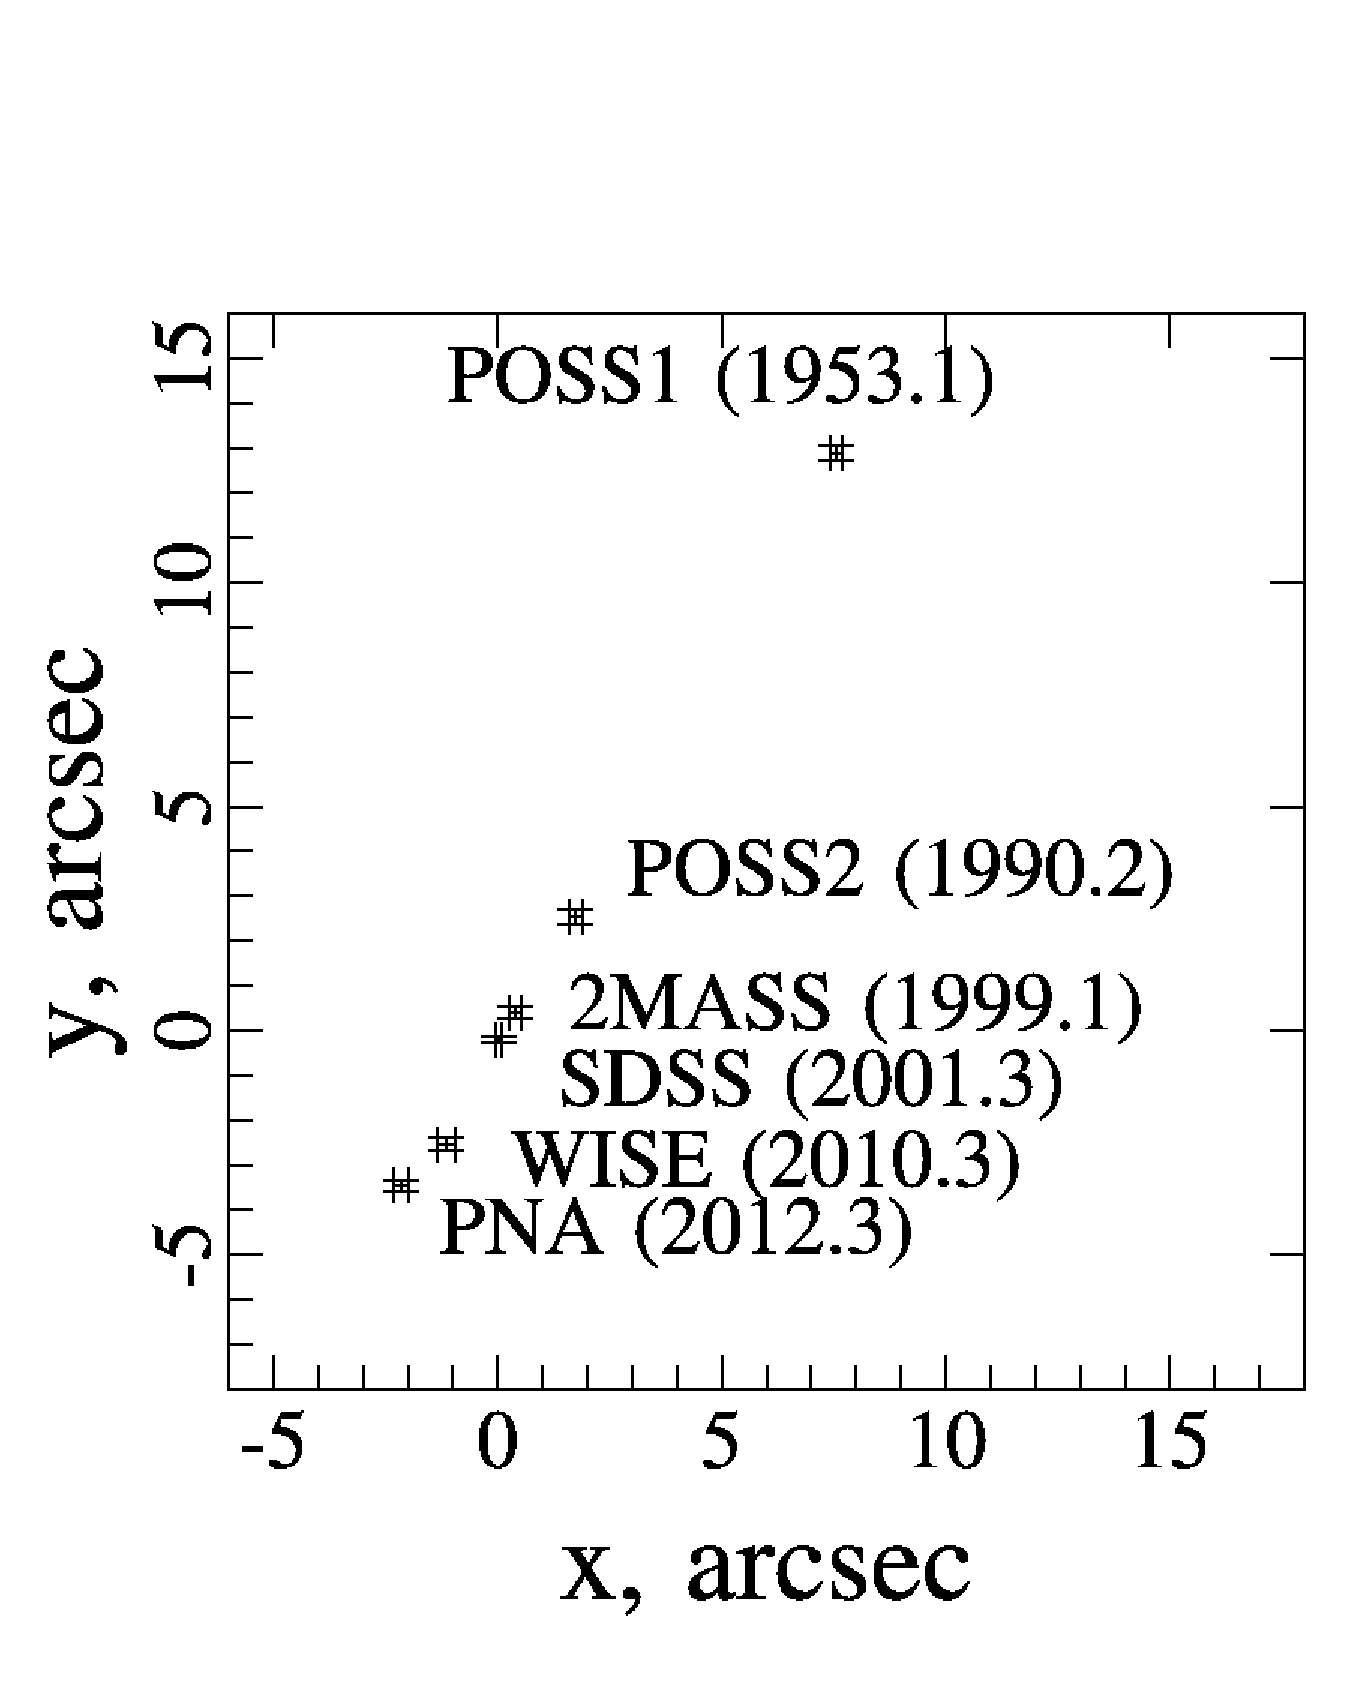
\includegraphics [scale=0.6] {fig6.eps}
\caption{Диаграмма движения звезды J0838+4715. Компоненты собственного движения составляют $-158.1\pm2.6$~mas/год по прямому восхождению и $-273.1\pm3.1$~mas/год по склонению. Средняя эпоха наблюдений "--- 1994.3328. $V_{mag} = 15.9$ (PNA - Пулковский Нормальный астрограф). Взято из работы \cite{2015AstL...41..833K}, рис.6.}
\label{fig:15j0838}
\end{figure}

\subsection{Вычисление порогового значения критерия для выявления $\Delta\mu$--двойных} \label{subsec:ch3/sect3/sub1}
Как упомянуто в первой главе, в работе Вилена и коллег \cite{1999A&A...346..675W} предложен статистический критерий, позволяющий решить, можно ли считать значимым различие квазисреднего ($\mu_{mean}$) и квазимгновенного ($\mu_{inst}$) собственных движений. В случае данных FK5 и Hipparcos собственные движения определялись на основе большого числа наблюдений, и сомнений в гауссовом характере распределения этих величин не было.

Величина F вычисляется по аналогии с формулой~\ref{eq:KhrF}: 
\begin{equation}
\label{eq:F2015}
F^2=\left(\frac{\Delta\mu_\alpha\cos\delta}{\varepsilon_{\mu_\alpha}}\right)^2 + \left(\frac{\Delta\mu_\delta}{\varepsilon_{\mu_\delta}}\right)^2,
\end{equation}
здесь $\Delta\mu_\alpha\cos\delta,~\Delta\mu_\delta$ "--- разности компонент собственного движения ($\mu_{mean}-\mu_{inst}$); $\varepsilon_{\mu_\alpha},~\varepsilon_{\mu_\delta}$ "--- соответствующие взаимные стандартные ошибки ($\varepsilon_\mu^2=\varepsilon_{\mu_{inst}}^2+\varepsilon_{\mu_{mean}}^2$).

Анализ интегрального распределения этой величины приводит к выводу, что при F>2.49 вероятность наблюдения соответствующих разностей собственных движений для одиночных звезд меньше 0.05. Именно такие звезды рассматривались в работе Вилена и коллег (Вилен и др., 1999) как кандидаты в $\Delta\mu$--двойные.

В нашем случае количество точек, по которым необходимо сделать вывод, невелико (от 4 до 10). Поэтому необходимо было проверить, можно ли использовать значение F=2.49 как пороговое. Для этого было предпринято численное моделирование линейного движения одиночной звезды по небесной сфере с заданными ошибками определения координат, охватывающего характерный для нашей задачи период времени (около 65 лет). Точки для определения собственных движений брались случайным образом, учитывая характерные времена осуществления используемых обзоров. Далее производились вычисления по схеме, описанной в предыдущем разделе, но для модельной звезды.

Рассматривались разные случаи: от 4 точек (есть два паломарских снимка, пулковские кадры и кадры 2MASS) до 10. Для каждого производилось 100000 испытаний. В результате для каждого случая строилось интегральное распределение величины F и вычислялось пороговое значение.

Как видно из графика на рисунке~\ref{fig:15Fint}, для 6 точек $F>5.3$, для 10 "--- $F>3.1$ и так далее. При увеличении до 20 точек пороговое приближается к 2.5. Что соответствует ситуации, рассмотренной в работе Вилена и коллег. Полученные таким образом пороговые значения использовались для реальных звезд, чтобы сделать вывод о характере движения звезды по небесной сфере.

\begin{figure}[h]
\centering
%\includegraphics [scale=1] {fig7.ps}
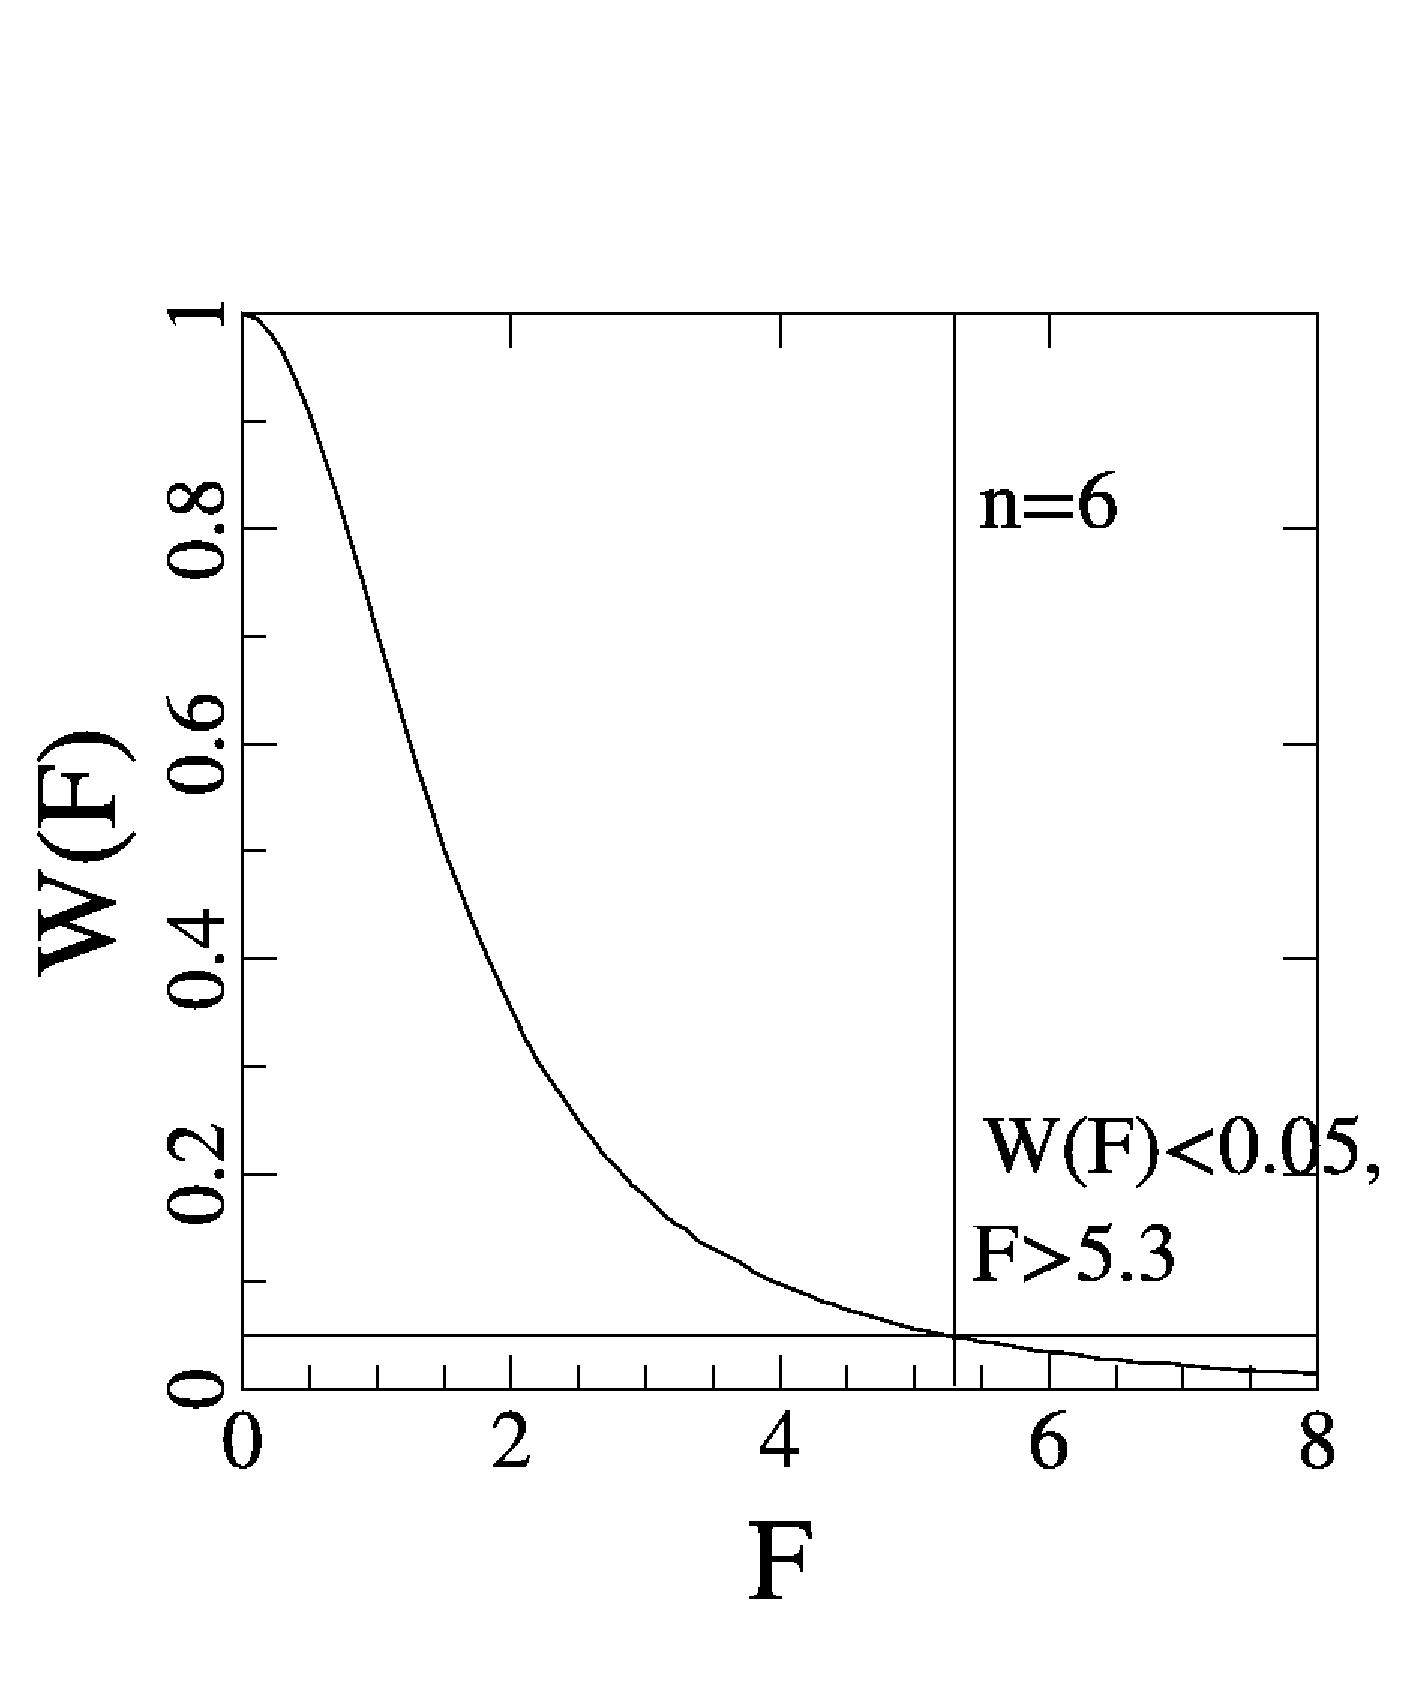
\includegraphics[width=0.49\columnwidth]{fig7a.eps}
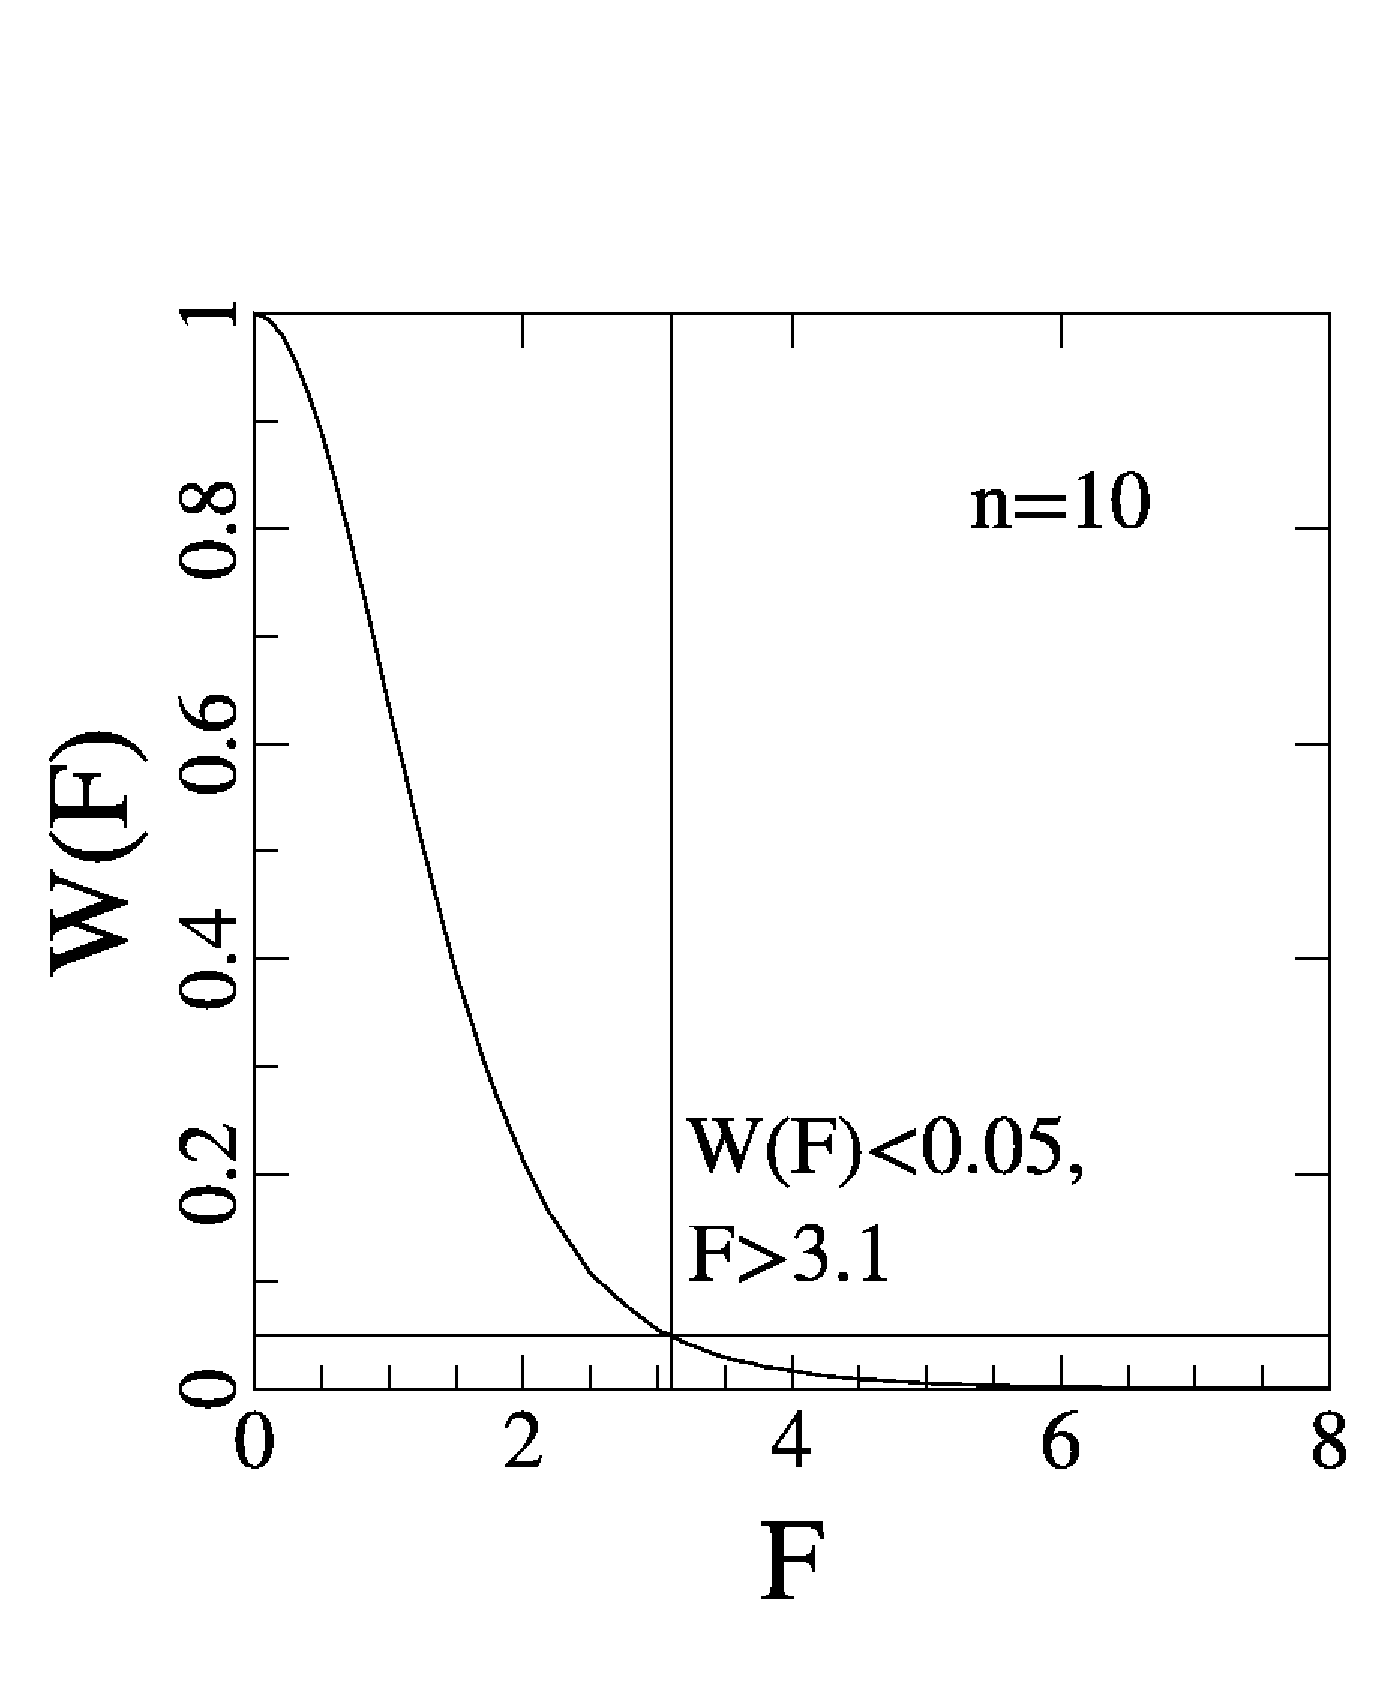
\includegraphics[width=0.49\columnwidth]{fig7b.eps}
\caption{Интегральные распределения величины F для разного числа кадров, использованных для вычисления собственных движений (слева n=6, справа n=10). Взято из работы \cite{2015AstL...41..833K}, рис.7.}
\label{fig:15Fint}
\end{figure}
\subsection{Общая характеристика полученных собственных движений} \label{subsec:ch3/sect3/sub2}
В конечном итоге с использованием описанной методики были обработаны кадры и сканы фотопластинок для 1308 звезд. Положения 120 звезд не удалось надежно измерить на кадрах ряда обзоров чаще всего из-за наличия рядом изображений очень ярких звезд. Для этих объектов требуются дополнительные исследования.

Все результаты собраны в 4 таблицы, доступные в электронном виде в базе данных CDS\footnote{\textit{(http://vizier.u-strasbg.fr/viz-bin/VizieR?-source=J/PAZh/41/896)}}. В качестве примера, небольшая часть основного массива данных показана в таблице~\ref{tab:candidates}. Для каждой звезды помимо собственных движений и оценок F-критерия, вычисленных в данной работе, приводятся дополнительные данные (разности собственных движений из сравнения с данными LSPM, фотометрические и тригонометрические параллаксы, оценки блеска для разных полос, принадлежность к каталогам двойных звезд). При формировании таблиц использовался сервис Центра астрономических данных в Страсбурге (Centre de Donnees astronomiques de Strasbourg) \cite{2000A&AS..143...23O}.

Надежность определения квазимгновенных собственных движений (третий вариант) существенно зависит от разности эпох между обзорами. Поэтому материал был разделен на две части. В первую из них вошли звезды, с соответствующей разностью эпох более 5~лет, все остальные "--- во вторую. В первой части оказалось 944 звезды, для которых не обнаружены признаки нелинейности движения, и 121 звезда, проявляющая себя как кандидат в $\Delta\mu$--двойные. Вторую группу составили 229 одиночных звезд  и 14 звезд--кандидатов в $\Delta\mu$--двойные.

Для собственных движений, построенных по всем обзорам (первый вариант), средняя точность составила чуть хуже 4~mas/год по обеим координатам. Для более полного представления о качестве собственных движений на рисунке~\ref{fig:15emu} приведены соответствующие гистограмма и зависимость ошибок определения собственных движений от блеска (для первого варианта собственных движений). Для подавляющего числа звезд ошибки определения собственных движений не превосходят 10~mas/год.

\begin{figure}[h]
\centering
%\includegraphics [scale=1] {fig8.ps}
\includegraphics[width=0.7\columnwidth]{fig8a.eps}\\
\includegraphics[width=0.7\columnwidth]{fig8b.eps}
\caption{Распределение ошибок собственных движений (сверху) и их зависимость от блеска (снизу). Взято из работы \cite{2015AstL...41..833K}, рис.8.}
\label{fig:15emu}
\end{figure}

Квазисредние собственные движения характеризуются средней точностью около 5~--~10~mas/год. Для квазимгновенных собственных движений эта величина составила 10~--~20~mas/год (она существенно зависит от наличия кадров SDSS и блеска звезды).

Наличие систематических различий между нашим набором собственных движений и собственными движениями звезд в каталоге LSPM демонстрирует рисунок~\ref{fig:15dmu}. Особенно эти различия заметны для собственных движений по склонению (разности могут достигать величины 2~--~4~mas/год).
\begin{figure}[h]
\centering
%\includegraphics [scale=1] {fig9.ps}
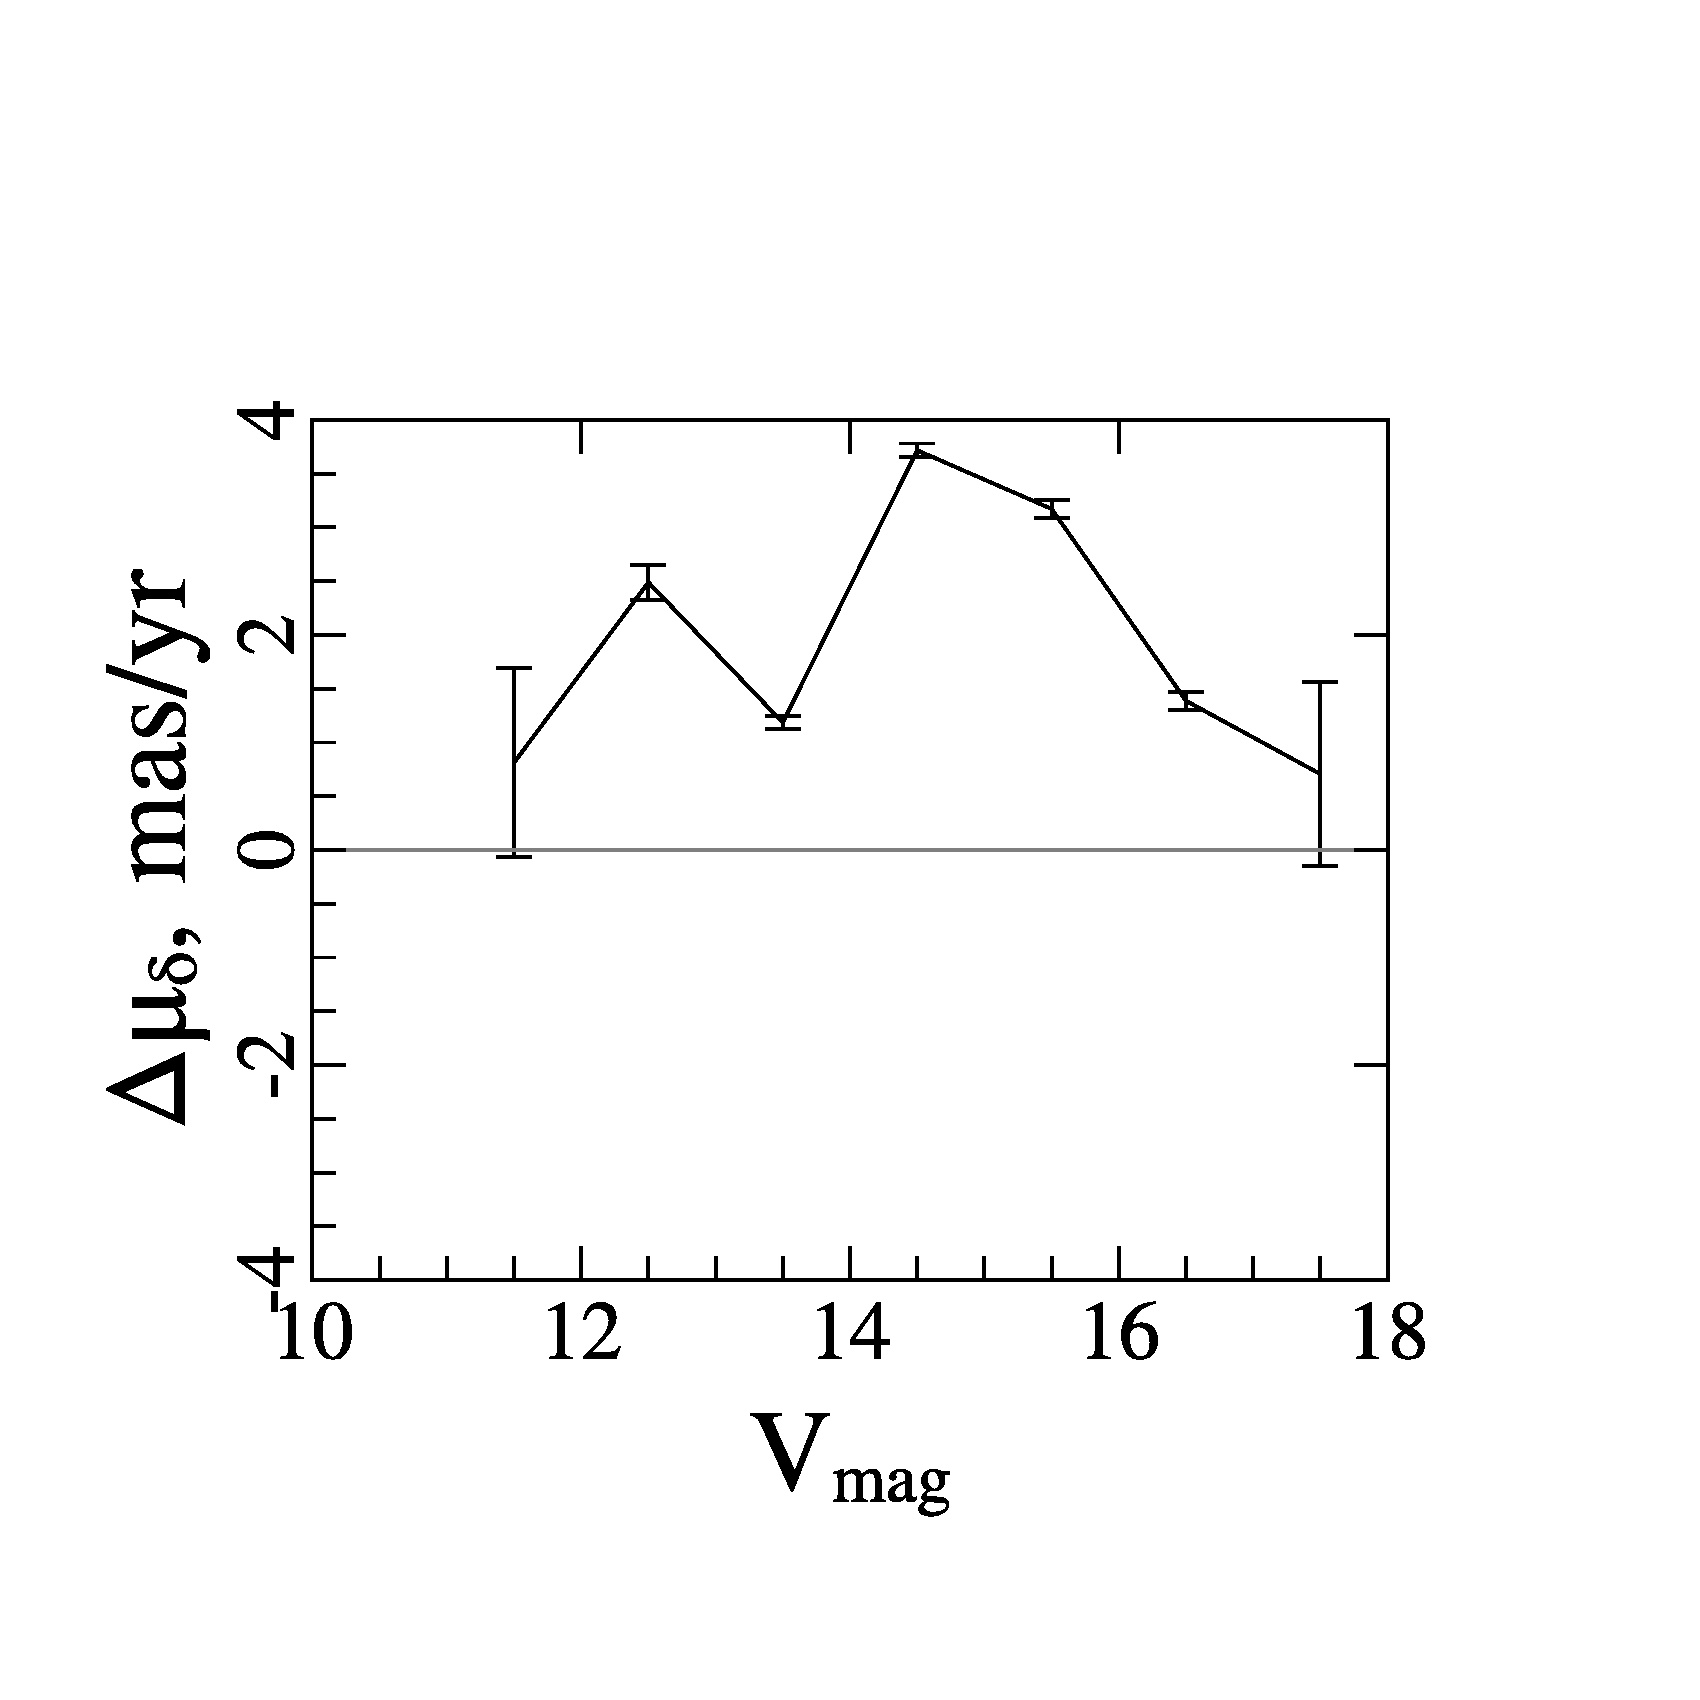
\includegraphics[width=0.7\columnwidth]{fig9a.eps}\\
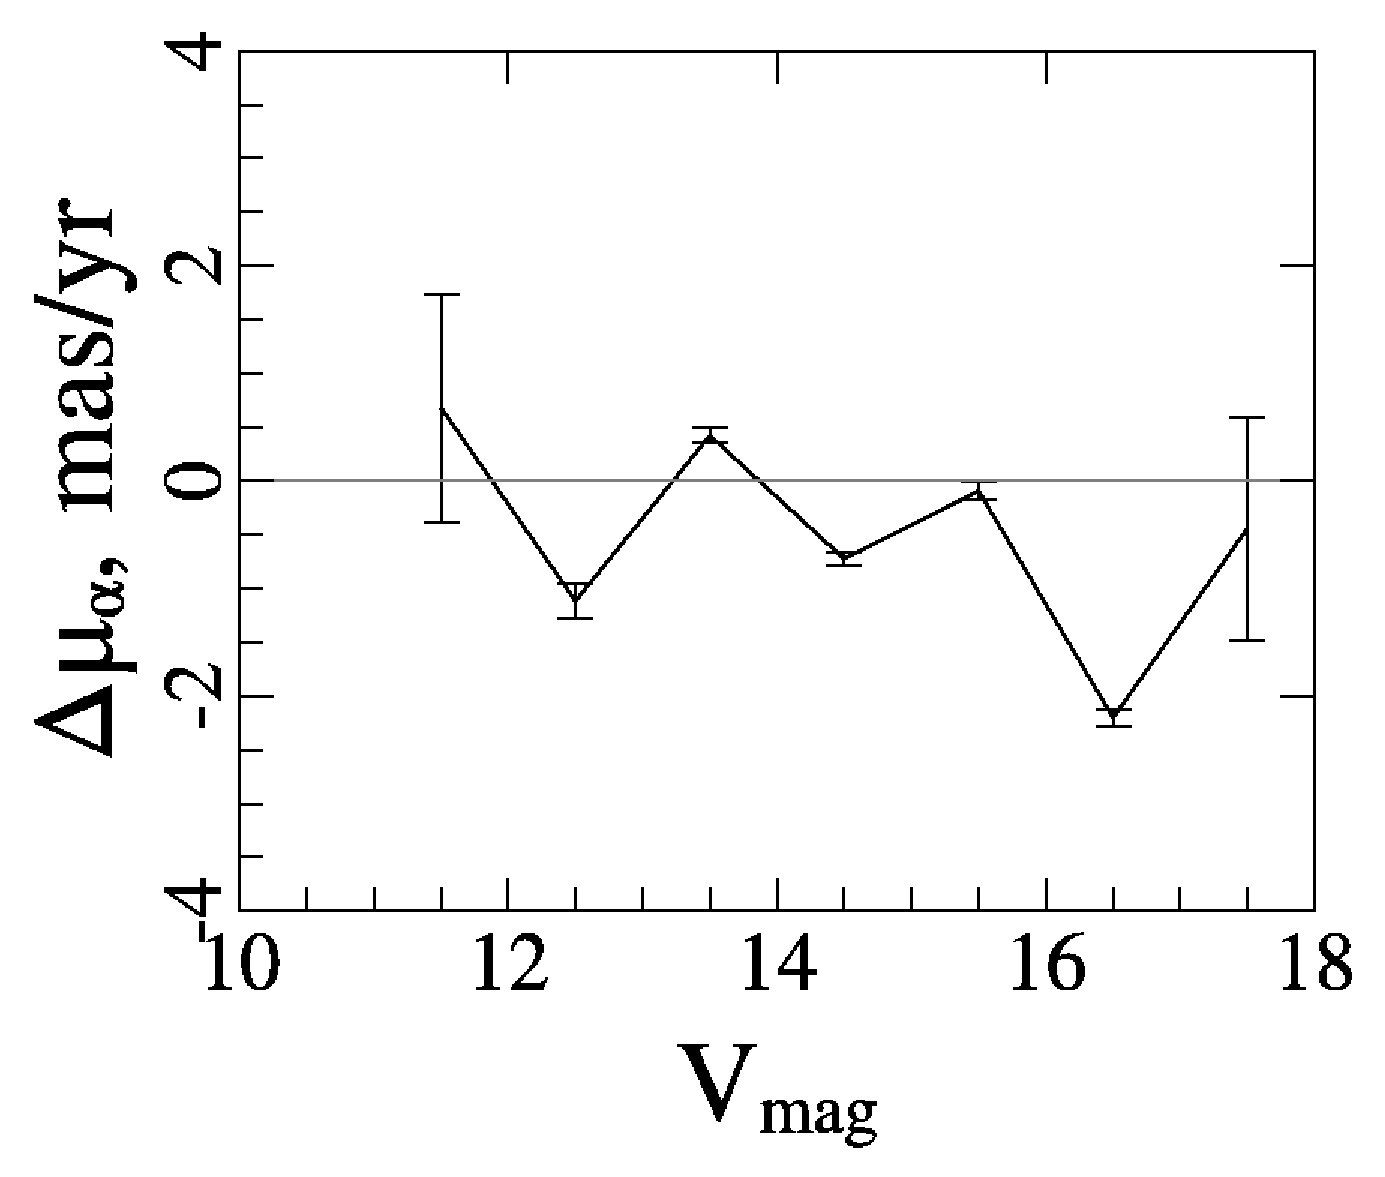
\includegraphics[width=0.7\columnwidth]{fig9b.eps}
\caption{Зависимость разностей собственных движений $\mu - \mu_{LSPM}$ от звездной величины ($\mu$ "--- собственное движение, вычисленное по всем кадрам). Взято из работы \cite{2015AstL...41..833K}, рис.9.}
\label{fig:15dmu}
\end{figure}
Особенность каталога LSPM состоит в нестандартном подходе к абсолютизации собственных движений. В период его создания слабые опорные звезды еще не были обеспечены надежными собственными движениями. Поэтому эта процедура производилась по ярким звездам каталога Tycho--2, изображения которых на пластинках паломарских обзоров либо передержаны, либо близки к этому. Экстраполяция абсолютизирующих поправок в область более слабых (на $3^m~--~5^m$) звезд никак не контролировалась, что, вероятно, стало причиной наблюдаемых систематических различий.
\subsection{Верификация выявленных звезд-кандидатов в $\Delta\mu$--двойные} \label{subsec:ch3/sect3/sub3}
Всего у 121 объекта обнаруживаются признаки нелинейности движения по небесной сфере, что классифицирует такие звезды как $\Delta\mu$--двойные. На наш взгляд, эти объекты представляют интерес для дальнейших исследований с целью подтверждения факта двойственности и определения орбит и масс посредством, например,  спекл--интерферометрических наблюдений на больших телескопах. Для 14 звезд из второй группы, для которых квазимгновенное собственное движение заметно отличается от квазисреднего, вывод о принадлежности к $\Delta\mu$--двойным представляется весьма ненадежным из-за малости разности эпох между положениями в современных обзорах неба. Поэтому дальнейший анализ касается только звезд первой группы.

Из нашего списка $\Delta\mu$--двойных 10 звезд входят в состав каталога WDS \cite{2001AJ....122.3466M}, то есть являются визуально--двойными звездами (это 9\,\% от общего числа $\Delta\mu$--двойных звезд). Большинство из них представляют собой широкие пары звезд с общим собственным движением (угловое разделение компонент составляет десятки угловых секунд, а в ряде случаев и минуты дуги). Данный результат является слабым подтверждением эффективности методики выявления $\Delta\mu$--двойных звезд. В списке из 944 \glqq одиночных\grqq\ звезд присутствует 58 вхождений в WDS (6\,\%). Поэтому нельзя говорить, что в списке  $\Delta\mu$--двойных доля известных визуально--двойных звезд значимо больше.

Часть звезд пулковской программы имеет тригонометрические параллаксы, полученные по наземным наблюдениям. Хорошо известно, что в ходе таких наблюдений совместно с параллаксами с высокой точностью определяются и величины собственных движений за короткий интервал времени (3~--~5 лет). Поэтому их можно рассматривать как квазимгновенные собственные движения и оценить величину $F_{\pi}$ из сравнения с собственным движением, определенным по итогам данной работы.

В нашем списке $\Delta\mu$--двойных оказалось 33 звезды, вошедших в параллактические программы. Из них 18 имеют величину $F_{\pi}>3$ (и пять звезд входят в WDS). Более детально о корреляции между независимыми наборами величин $F$ и $F_\pi$ можно судить по рисунку~\ref{fig:15FF}. С некоторой натяжкой можно говорить о наличии корреляции между $F$ и $F_\pi$ для $\Delta\mu$--двойных. В случае звезд, которые рассматриваются как \glqq одиночные\grqq\ признаки корреляции не столь заметны. Положения визуально-двойных звезд из каталога WDS помечены на рисунке~\ref{fig:15FF} незакрашенными символами. Они есть как среди $\Delta\mu$--двойных, так и в числе \glqq одиночных\grqq\ звезд. И это вполне естественно. Для широких пар с большими периодами обращения (сотни и тысячи лет), которых довольно много в нашем материале, орбитальное движение очень непросто обнаружить на используемом ряде наблюдений.
\begin{figure}[h]
\centering
 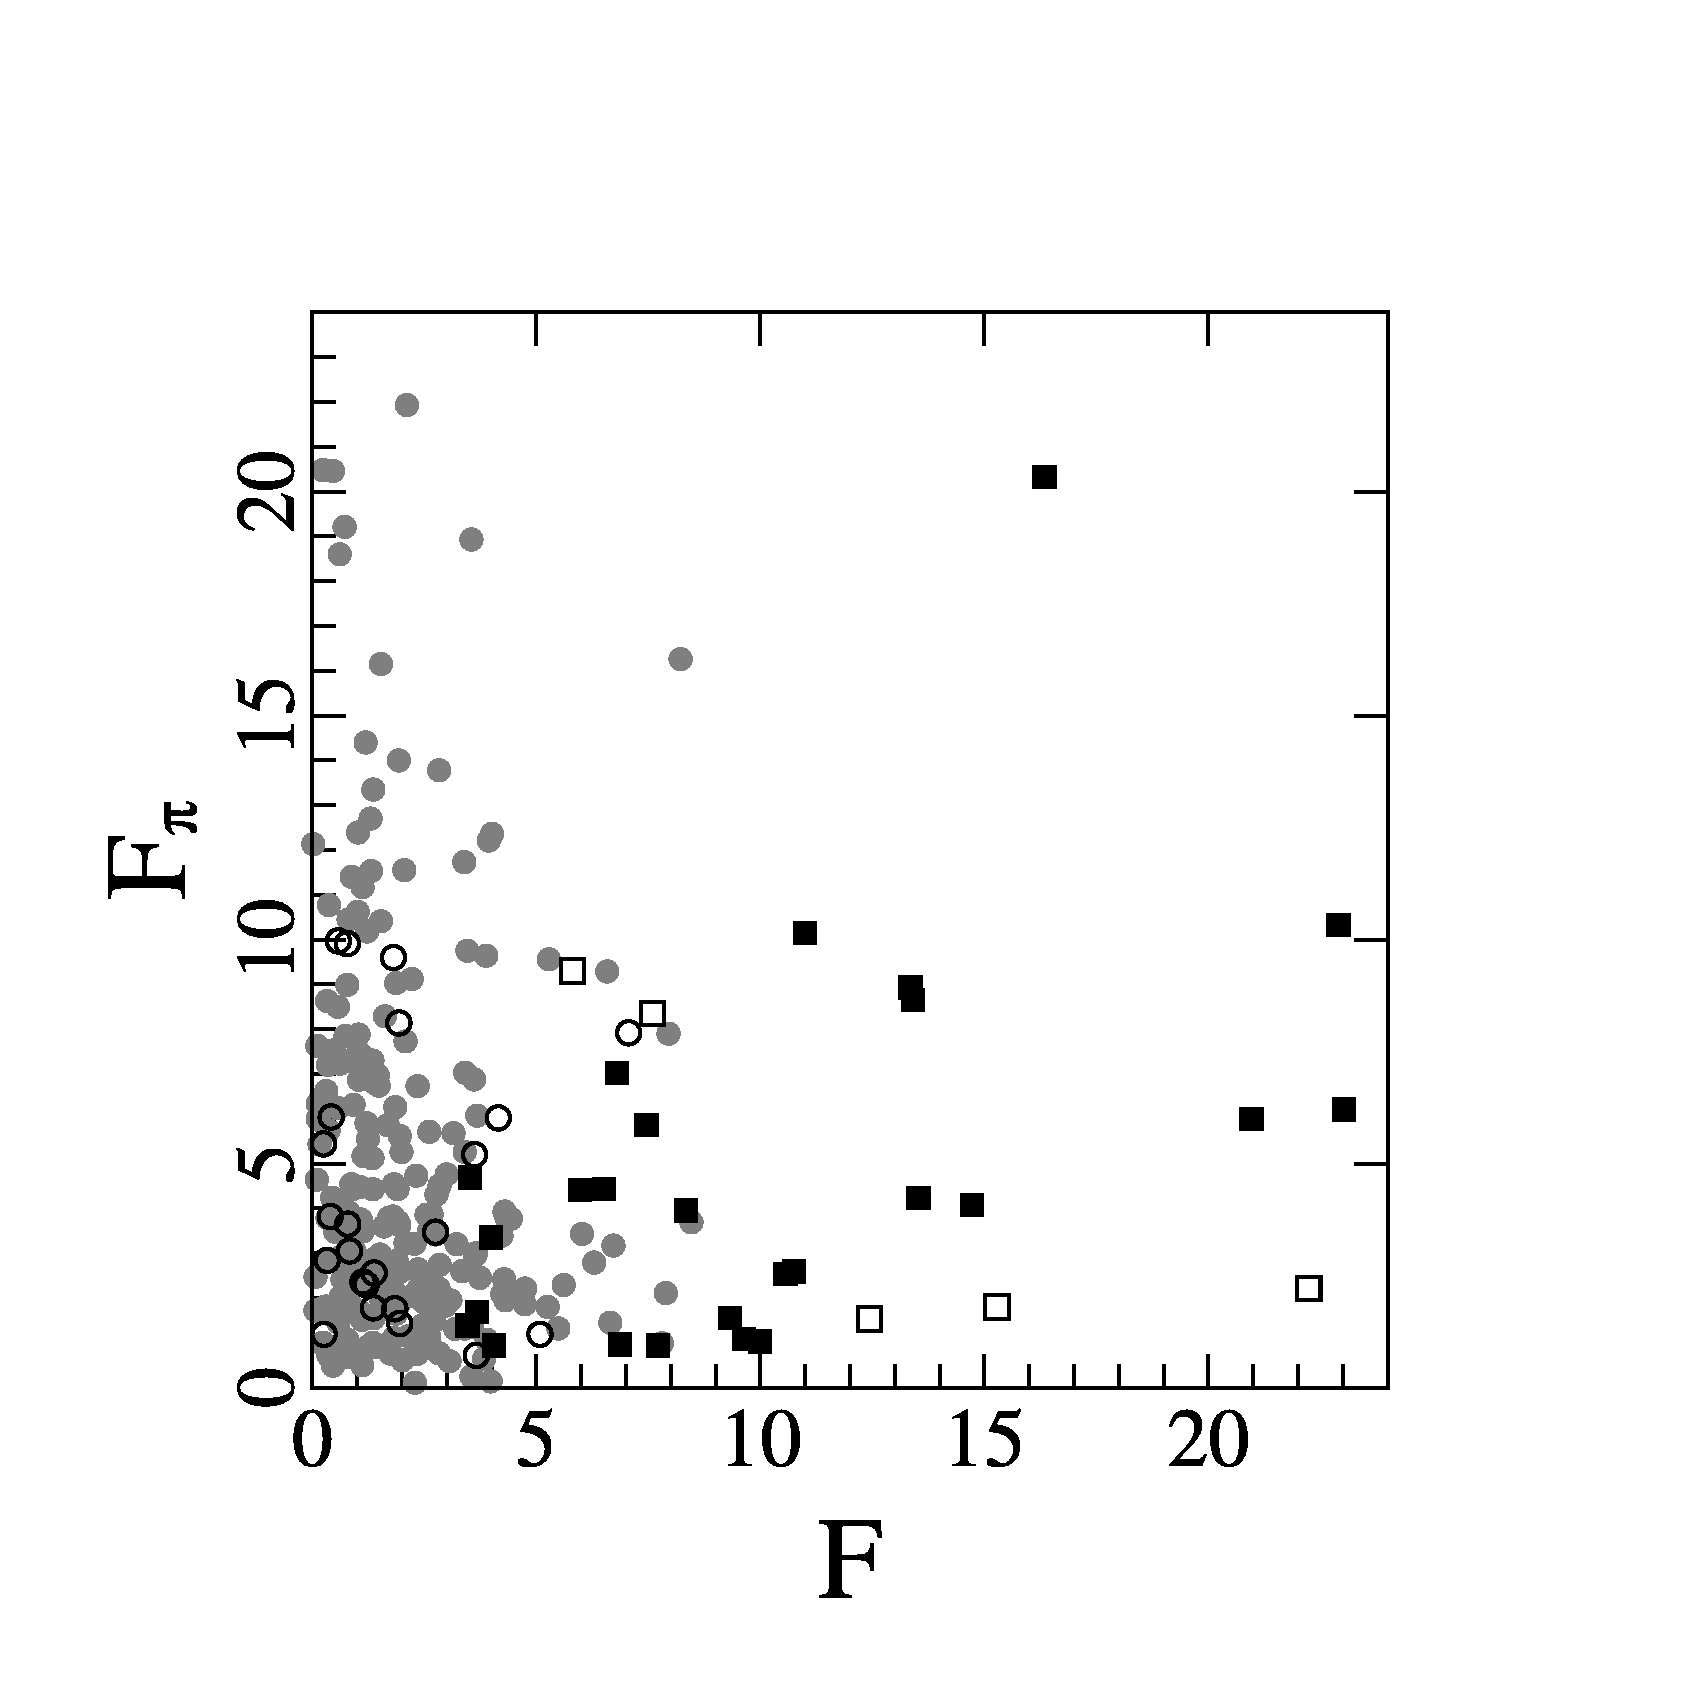
\includegraphics [scale=0.6] {fig10.eps}
\caption{Распределение звезд на плоскости $F-F_{\pi}$. $F$ "--- значения критерия, полученные из анализа ПЗС-кадров и сканов обзоров. $F_{\pi}$ определялись на основе собственных движений из данной работы и собственных движений, полученных в ходе реализации различных параллактических программ (кружки обозначают \glqq одиночные\grqq\ звезды, квадраты "---  $\Delta\mu$--двойные; символы, отвечающие звездам из каталога WDS, не закрашены). Взято из работы \cite{2015AstL...41..833K}, рис.10.}
\label{fig:15FF}
\end{figure}

Для близких к Солнцу двойных систем карликовых звезд угловые расстояния между компонентами могут составлять секунду дуги и более. Поэтому факт двойственности может быть установлен просто из анализа изображений звезд на ПЗС--кадрах. Shapelet--разложение, использованное для определения пиксельных координат звезд, позволяет оценивать такой параметр как асимметрия изображения. Для того, чтобы понять насколько надежен такой подход, было выполнено численное моделирование изображений подобных пар. Для обзора SDSS, который обладает наилучшим \glqq разрешением\grqq\ среди всех использованных обзоров, на основе результатов аппроксимации изображений одиночных звезд строились модельные \glqq взаимодействующие\grqq\ изображения для систем с характерными значениями блеска компонент при разных угловых расстояниях между ними. Затем эти \glqq взаимодействующие\grqq\ изображения снова подвергалось Shapelet--разложению. Пример зависимости асимметрии от углового расстояния для пары с блеском компонент $14.1^m$ и $15.3^m$ показан на рисунке~\ref{fig:15asimm}. Анализ этого графика дает основания говорить, что оценки асимметрии изображений наиболее эффективны для угловых расстояний 2~--~4 угловых секунды. Асимметрия заметна и для меньших разделений, но для оценки надежности рассматриваемого подхода для таких \glqq тесных пар\grqq\ требуются дополнительные исследования. Учитывая качество изображений и масштабы ПЗС-кадров и сканов из остальных использованных обзоров можно заключить, что оценок асимметрии изображений недостаточно для установления факта двойственности. Тем не менее, величины асимметрии весьма информативны для анализа вместе с оценками F--критерия. Поэтому в финальную таблицу с результатами включены средние величины асимметрии по всем обзорам, приведены максимальные величины асимметрии по всей выборке для данной звезды с указанием соответствующего обзора (таблица~\ref{tab:candidates}). Любопытно отметить, что для выборки $\Delta\mu$--двойных звезд средняя асимметрия звездных изображений составляет 0.039. Для \glqq одиночных\grqq\ звезд этот показатель составил 0.025.
\begin{figure}[h]
\centering
 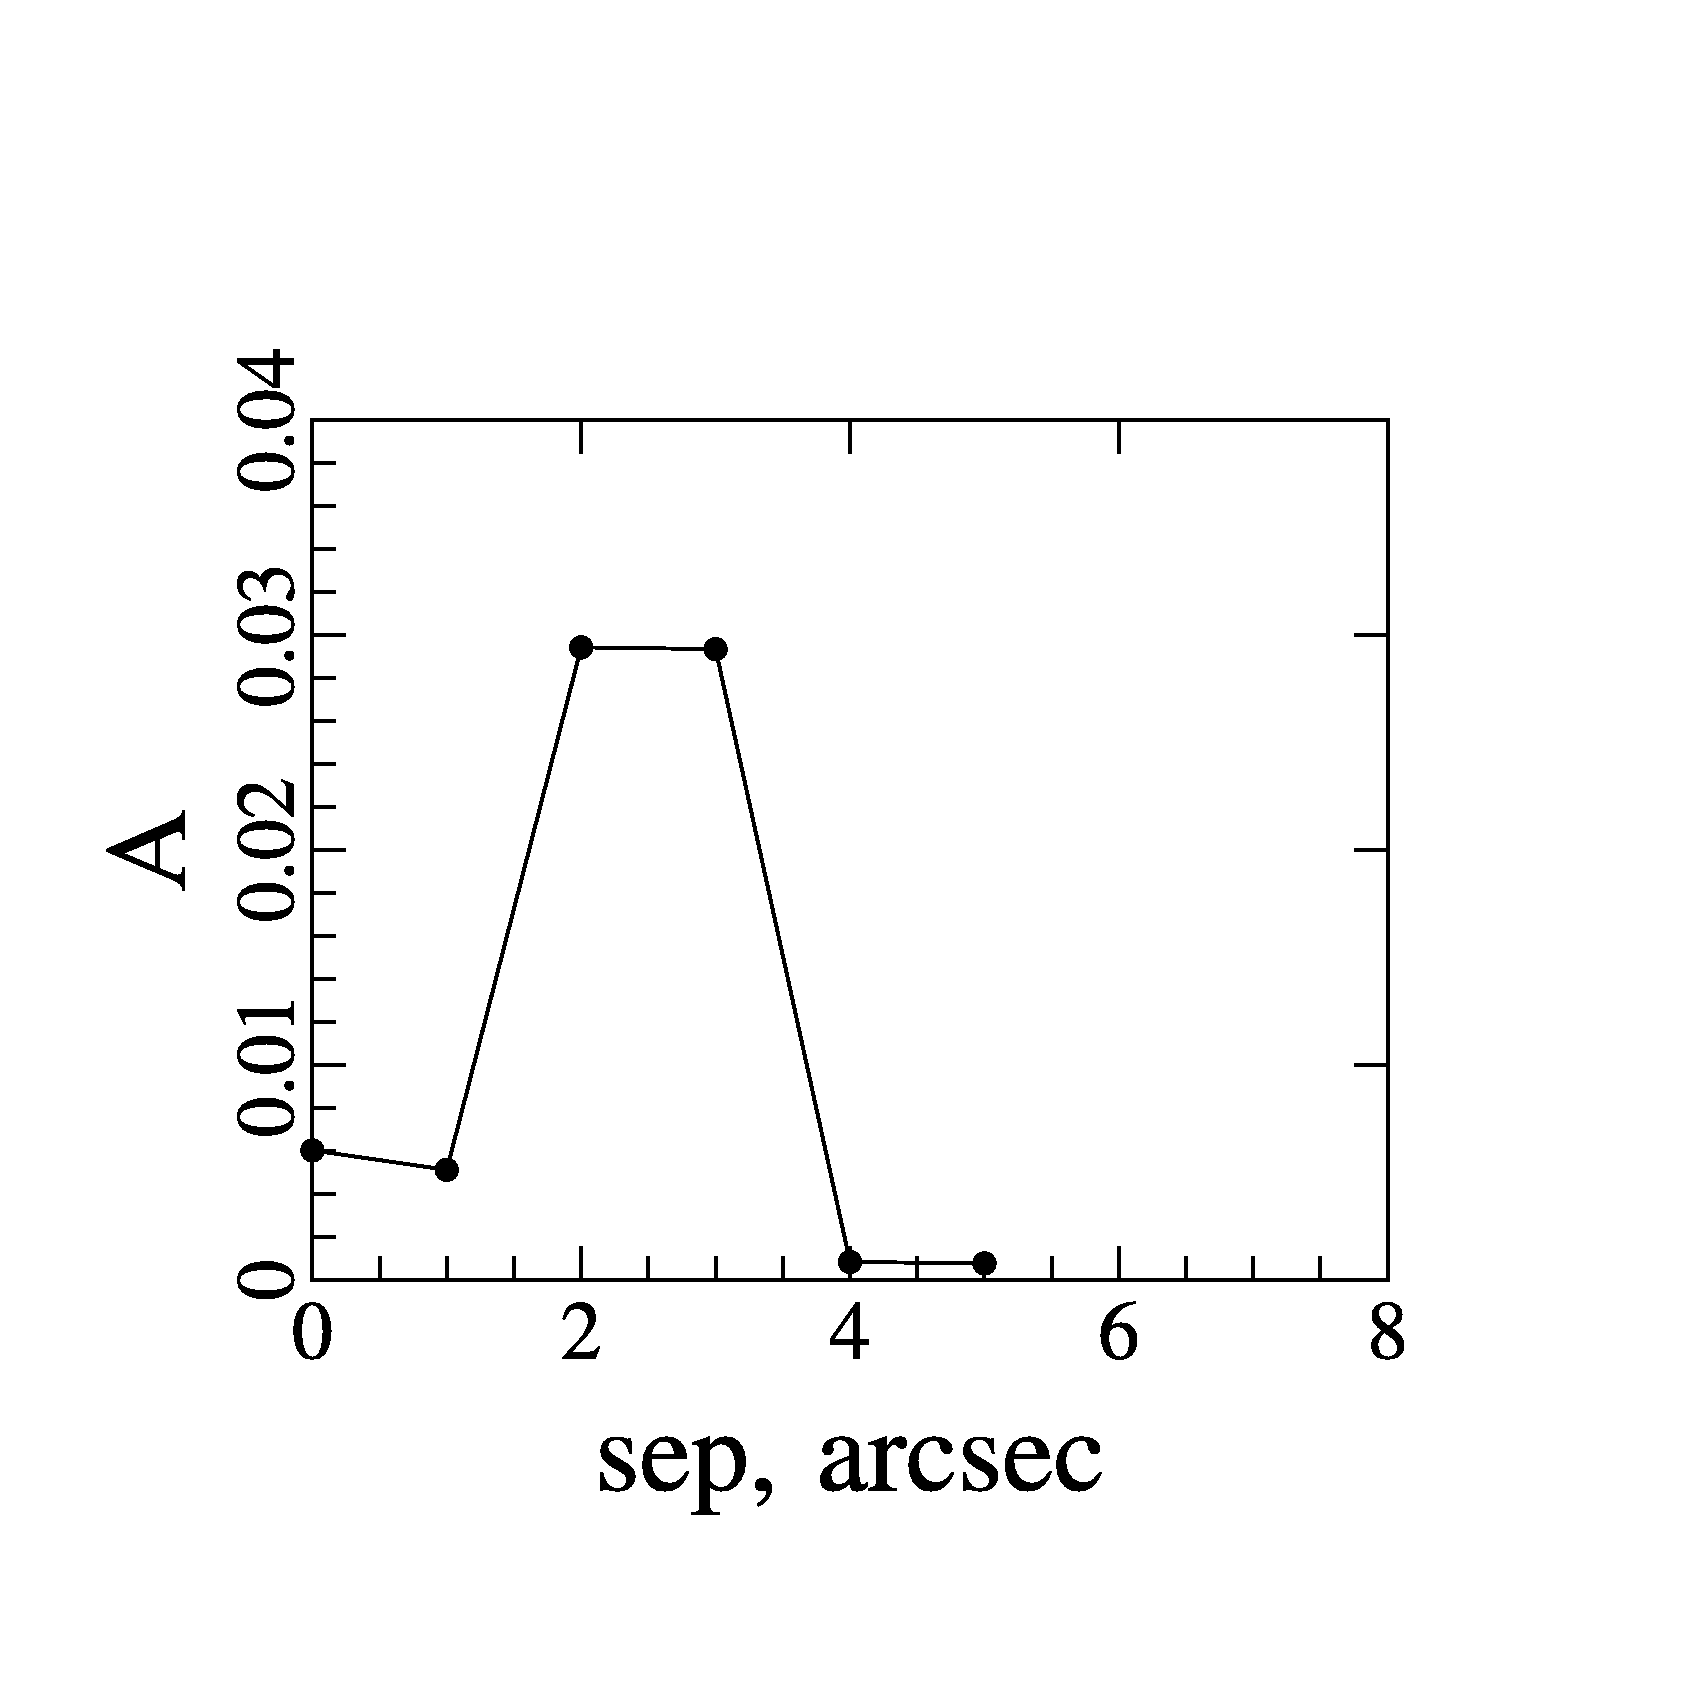
\includegraphics [scale=0.6] {fig11.eps}
\caption{Симуляция зависимости асимметрии взаимодействующих изображений звезд от углового расстояния между звездами (главная компонента "--- $14.1^m$, вторая звезда "--- $15.3^m$). За основу были взяты результаты shapelet--разложений звезд на кадрах обзора SDSS. Взято из работы \cite{2015AstL...41..833K}, рис.11.}
\label{fig:15asimm}
\end{figure}

Параметры двойных систем из каталога WDS (разделение между компонентами, позиционные углы, блеск компонент) включены в электронные версии таблиц с результатами. Для $\Delta\mu$--двойных звезд J0027+5330N, J0514+4431N, J0517+4550, J1614+6038, J1938+3512E угловые разделения между компонентами лежат в пределах от долей угловой секунды до $4''$. Звезда J1938+3512E входит в обзор SDSS и имеет асимметрию 0.086, что заметно выше средних показателей для \glqq одиночных\grqq\ звезд того же блеска в этом обзоре (обычно от 0 до 0.04). Эти звезды можно выделить как примеры успешного детектирования нелинейного движения по небесной сфере на основе сравнения квазисреднего и квазимгновенного собственных движений.

Положения фотоцентров изображений рассматриваемых двойных систем могут отличаться в зависимости от эффективной длины волны в случае заметной разности эффективных температур компонент (например, для систем типа \glqq М--карлик + коричневый карлик\grqq ). Если бы обзоры выполнялись одновременно, можно было бы легко обнаружить этот факт, сравнивая координаты звезд и выделяя заметные смещения центров изображений от \glqq оптических\grqq\ к \glqq инфракрасным\grqq\ обзорам. Космический обзор WISE более современный и более глубокий по сравнению с 2MASS. Но в астрометрическом отношении обзор 2MASS значительно более качественный (ошибки астрометрической редукции для WISE могут достигать 100~--~200~mas, для 2MASS они, как правило, меньше 50~mas). Поэтому если число положений звезды в \glqq оптических\grqq\ обзорах (POSS1, POSS2, SDSS, PNA) было не менее четырех, вычислялся вариант собственного движения только по данным \glqq оптических\grqq\ обзоров. С помощью этого собственного движения вычислялось \glqq оптическое\grqq\ положение звезды на эпоху обзора 2MASS. В результате можно было оценить смещение ($\rho$) между \glqq оптическим\grqq\ положением и положением в обзоре 2MASS. Если $\rho>5\sigma$, величина смещения и его отношение к взаимной ошибке координат приводится в финальной таблице. Например, звезда J1931+4115 (таблица~\ref{tab:candidates}). Для нее смещение превосходит $1''$. Асимметрия изображения для этой звезды близка к средней по выборке $\Delta\mu$--двойных звезд и больше средней для \glqq одиночных\grqq . Такой совместный анализ множества критериев позволяет заключить, что предложенная методика поиска $\Delta\mu$--двойных звезд является эффективной для определенного класса двойных систем среди звезд низкой светимости.

Еще одна возможность верификации детектирования $\Delta\mu$--двойных связана с анализом фотометрических данных. Самые точные из доступных для выявленных звезд оценок блеска присутствуют в SDSS (это величины u,\,g,\,r,\,i,\,z). Используя безансонскую модель Галактики \cite{2003A&A...409..523R} и падуанские изохроны\footnote{\textit{http://stev.oapd.inaf.it/cgi-bin/cmd}} (\cite{2012MNRAS.427..127B}, \cite{2014MNRAS.444.2525C}, \cite{2014MNRAS.445.4287}), были построены двухцветные диаграммы (g--z)~--~(u--g) для звезд с массами от 0.1 до 0.7 массы Солнца. Техника построения диаграмм полностью аналогична методике, ранее использованной при реализации пулковской программы изучения звезд с большими собственными движениями \cite{2013MNRAS.435.1083K}.

Чтобы понять, как смешение цветов неразрешенных звездных пар влияет на распределение плотности, с которой звезды заполняют пространство (g--z)~--~(u--g), строились диаграммы как для одиночных звезд, так и с учетом различных комбинаций компонент двойных систем в зависимости от масс и возрастов (при этом считалось, что доля двойных звезд составляет 0.5).  Положения выявленных звезд-кандидатов в $\Delta\mu$--двойные на диаграммах для одиночных (слева) и с учетом доли двойных звезд (справа) показаны на рисунке~\ref{fig:15color}.

\begin{figure}[h]
\centering
%\includegraphics [scale=1] {fig12.ps}
\includegraphics[width=0.6\columnwidth]{fig12a.eps}\\
\includegraphics[width=0.6\columnwidth]{fig12b.eps}
\caption{Положения звед--кандидатов в $\Delta\mu$-двойные на двухцветной диаграмме $(g-z)$~--~$(u-g)$. На рисунке показаны теоретические последовательности для звезд в диапазоне от 0.1 до 0.7 массы Солнца, построенные на основе падуанских изохрон и безансонской модели Галактики для одиночных звезд (сверху) и при добавлении двойных систем типа  \glqq M--карлик + белый карлик\grqq\ (снизу). Массы белых карликов составляют 0.3 и 0.6 массы Солнца (возрасты 0.6 и 1 млрд. лет соответственно). Черные квадраты соответствуют звездам, которые могут оказаться системами  \glqq M--карлик + белый карлик\grqq . Шкала справа показывает значение натурального логарифма относительной плотности распределения модельных звезд на диаграмме. Взято из работы \cite{2015AstL...41..833K}, рис.12.}
\label{fig:15color}
\end{figure}

Метод поиска $\Delta\mu$--двойных максимально эффективен при большом различии положений центра масс и фотоцентра двойной системы. Поэтому большой интерес вызывает поиск пар \glqq M--карлик + белый карлик\grqq , для которых отношение светимостей компонент заметно больше отношения масс. Модельные расчеты показали, что для большинства комбинаций M--карликов разных масс отклонения от основного массива точек на диаграмме (g--z)~--~(u--g) незаметны. В то время как пары \glqq M--карлик + белый карлик\grqq\ могут дать заметный эффект. Чтобы оценить его наглядно, для примера, были взяты модели белых карликов  с массами 0.3 и 0.6 массы Солнца и возрастами 0.6 и 1 млрд. лет (\cite{2006AJ....132.1221H}, \cite{2011ApJ...737...28B}, \cite{2006ApJ...651L.137K}, \cite{2011ApJ...730..128T})\footnote{\textit{http://www.astro.umontreal.ca/~bergeron/CoolingModels/}}. Смешение цветов данных белых карликов с цветами M--карликов разных масс и соответствующих возрастов (с учетом того, что белые карлики прошли прошли фазу эволюции на главной последовательности) обуславливает отличие вида диаграмм на левой и правой панелях рисунка~\ref{fig:15color}.  Анализ отклонений $\Delta\mu$--двойных от основного массива точек на этом рисунке дает основания для вывода о том, что 4 звезды (J0656+3827, J0838+3940, J1229+5332, J2330+4639 "--- обозначены квадратными метками) могут рассматриваться как возможные пары такого типа.

Подробная информация об этих четырех звездах приведена в таблице~\ref{tab:MDWD}. Три звезды из четырех характеризуются большими ($>0.1$) значениями асимметрии звездных изображений, полученными при анализе ПЗС-кадров обзора SDSS. Привлекает внимание звезда J2330+4639, входящая в WDS как сравнительно широкая пара (разделение компонент 21.4$''$). Для этой звезды очень сильно отличаются квазимгновенные и квазисредние собственные движения при очень большой асимметрии (0.244). Это можно объяснить как следствие \glqq взаимодействия\grqq\ изображений двух близко расположенных звезд, что могло стать причиной систематической ошибки определения координат звезды в одном из современных обзоров. При анализе этой информации следует иметь ввиду, что в плотных звездных полях (когда на небольшом участке кадра в несколько минут дуги наблюдаются десятки звезд) близкие к Солнцу и быстро летящие звезды способны располагаться очень тесно к звездам фона на кадрах отдельных обзоров. Поэтому возможно формирование \glqq взаимодействующих\grqq\ изображений в ситуации, когда речь не может идти о двойной звезде. Однако проверить это пока довольно сложно, из-за того, что использованные обзоры имеют разную предельную звездную величину.

Итак, материал этой главы демонстрирует, что метод детектирования $\Delta\mu$--двойных, разработанный изначально для анализа звезд с \glqq хорошей\grqq\ астрометрической историей, был модифицирован для исследвоания собственных движений объектов, имеющих лишь несколько надежных положений. Это позволило установить, что более 100 звезд, относящихся к категории маломассивных карликов солнечной окрестности, могут рассматриваться как кандидаты в двойные системы. Это позволяет более адресно организовать проверку факта двойственности с помощью методов высокого разрешения. Как было показано, рационально принимать во внимание не только факт значимых различий собственных движений, но и свойства изображений звезд на ПЗС--кадрах (из формы). Этот подход будет более подробно изложен в дальнейшем тексте.

\begin{table}[htbp]
%\vspace{6mm}
%\small
\centering
\caption{Фрагменты таблицы для звезд-кандидатов в $\Delta\mu$--двойные.  Взято из работы \cite{2015AstL...41..833K}, таб.1.}
\label{tab:candidates}
\vspace{5mm}
\begin{tabularx}{\textwidth}{l|r|r|r|r|r|r|r|r|l} \hline
           & \multicolumn{4}{c|}{Квазисреднее $\mu$ } & \multicolumn{4}{c|}{Квазимгновенное $\mu$}& \\ \cline{2-9}
\multicolumn{1}{c|}{LSPM}&\multicolumn{1}{c|}{$\mu_\alpha$}&\multicolumn{1}{c|}{$\mu_\delta$}&\multicolumn{1}{c|}{$\varepsilon_{\mu_\alpha}$}&\multicolumn{1}{c|}{$\varepsilon_{\mu_\delta}$}&\multicolumn{1}{c|}{$\mu_\alpha$}&\multicolumn{1}{c|}{$\mu_\delta$}&\multicolumn{1}{c|}{$\varepsilon_{\mu_\alpha}$}&\multicolumn{1}{c|}{$\varepsilon_{\mu_\delta}$}&\multicolumn{1}{c}{T}\\ \cline{2-9}	   
	       &\multicolumn{8}{c|}{mas/yr}&\\ \hline  
J1756+5132 & -526.8&  205.3&  5.3&  5.2& -457.7&  -19.4& 17.1& 18.2& 2007.0035\\
J1844+6511 &  -16.5&  356.4&  7.1&  5.4&   30.0&  289.0&  0.3&  3.7& 2005.4087\\
J1908+3216 & -238.5& -227.0&  6.8&  6.3& -200.9& -215.4&  0.5&  9.5& 2006.9105\\
J1931+4115 & -249.7& -119.4& 15.6& 14.1& -329.5&   -1.4&  7.9&  4.4& 2007.7614\\
J1931+6843 &  256.2&  461.7&  6.3&  4.9&  228.9&  349.9&  5.8&  0.4& 2006.9060\\
J1938+3512E&   -2.1&  814.7& 11.4& 12.2& -123.3&  714.9&  6.1&  0.3& 2004.6930\\ \hline
\end{tabularx}
\begin{tabularx}{\textwidth}{l|r|c|r|r|r|r|r|r|l}

\multicolumn{1}{c|}{LSPM}&\multicolumn{1}{c|}{F}&\multicolumn{1}{c|}{n}&\multicolumn{1}{c|}{$V_{mag}$}&\multicolumn{1}{c|}{{\small$V$--$J$}}&\multicolumn{1}{c|}{$\rho$,mas}&\multicolumn{1}{c|}{$\rho/\varepsilon$}&\multicolumn{1}{c|}{$\langle A\rangle\ $}&\multicolumn{1}{c|}{$A_{max}$}& \multicolumn{1}{c}{Обзор}\\ \hline
        J1756+5132 & 12.50& 4 & 15.96& 3.18 &     &     & 0.040& 0.080& poss1\\
J1844+6511 & 12.23& 5 & 16.46& 4.08 &     &     & 0.026& 0.060& poss2\\
J1908+3216 &  5.57& 6 & 11.83& 3.92 &     &     & 0.019& 0.045& wise\\
J1931+4115 &  9.18& 7 & 12.20& 2.12 & 1241&  5.7& 0.032& 0.080& poss2\\
J1931+6843 & 22.90& 5 & 14.67& 4.65 &     &     & 0.027& 0.050& poss1\\
J1938+3512E& 12.44& 5 & 14.75& 2.98 &     &     & 0.038& 0.086& sdss\\
\hline
\end{tabularx}
\begin{flushleft}
\footnotesize
\textbf{Примечание.} $\mu_{\alpha}$, $\mu_{\delta}$, $\varepsilon_{\mu_{\alpha}}$, $\varepsilon_{\mu_{\delta}}$ "--- компоненты собственного движения и их стандартные ошибки.\\T "--- средняя эпоха для квазимгновенного собственного движения.\\F "--- величина критерия \glqq нелинейности\grqq\ движения звезды.\\ n "--- число использованных обзоров.\\ $V_{mag}$, {\small$V$--$J$} "--- звездная величина и показатель цвета. \\ $\rho$ "--- угловое расстояние между \glqq оптическими\grqq\ и \glqq ИК\grqq\ положениями фотоцентра. \\ $\rho/\varepsilon$ "--- отношение $\rho$ к стандартной ошибке ($\varepsilon$) определения координат звезды. \\ $\rho$ и $\rho/\varepsilon$ приводятся, только если $\rho/\varepsilon>5$. \\ $\langle A\rangle\ $"--- среднее значение \glqq асимметрии\grqq\ изображения звезды по всем обзорам. \\ $A_{max}$ "--- максимальное значение \glqq асимметрии\grqq\ изображения звезды и название соответствующего обзора. \\ Звезда J1938+3512E входит в каталог WDS (19389+3512, угловое разделение $\rho=4''$, позиционный угол: $PA=77^{\circ}$, блеск главной компоненты: $mag_p = 15.3$, блеск второй компоеннты: $mag_s=16.00$).
\end{flushleft}
\end{table}




\begin{table}[t]
\vspace{6mm}
\centering
\caption{Вероятные пары \glqq M--карлик~+~белый карлик\grqq . Взято из работы \cite{2015AstL...41..833K}, таб.2.}
\label{tab:MDWD}
\vspace{5mm}

\begin{tabularx}{\textwidth}{c|c|c|r|r|c} 
\hline
\multirow{2}{*}{LSPM} & $\alpha_{J2000}$ & $\delta_{J2000}$ &\multicolumn{1}{c|}{$\mu_\alpha$}&\multicolumn{1}{c|}{$\mu_\delta$}& \multirow{2}{*}{T} \\ \cline{2-5}
& $^h$~$^m$~$^s$  & $^\circ~'~''$ & \multicolumn{2}{c|}{mas/yr} & \\ \hline
J0656+3827 & 06:56:15.9901 & +38:27:45.954 &   320.5 & -105.9 & 1995.8213 \\
           & 61            & 68            &     4.5 &    5.4 & \\
J0838+3940 & 08:38:16.7026 & +39:40:49.250 &   157.1 &  107.6 & 1994.1300 \\
           & 102           & 157           &     5.5 &    8.9 & \\
J1229+5332 & 12:29:15.5864 & +53:32:43.762 & -1231.7 &  139.8 & 1991.6092 \\
           & 38            & 7             &     2.8 &    0.9 & \\
J2330+4639 & 23:30:41.5392 & +46:39:56.627 &   483.7 &  -90.7 & 1995.3407 \\
           & 124           & 198           &     6.6 &   14.8 & \\ \hline
\end{tabularx}
\begin{flushleft}
\footnotesize     
Здесь $\mu_\alpha$,$\mu_\delta$ "--- компоненты собственного движения, вычисленного по всем обзорам. Вторая строчка для каждой звезды содержит стандартные ошибки координат (в mas) и собственных движений (mas/yr).
\end{flushleft}
%\vspace{5mm}
\begin{tabularx}{\textwidth}{l|r|r|r|r|r|r|r|r|c} \hline
     & \multicolumn{4}{c|}{квазисреднее $\mu$ }
     &\multicolumn{4}{c|}{квазимгновенное $\mu$}&  \\ \cline{2-9}
\multicolumn{1}{c|}{LSPM}&\multicolumn{1}{c|}{$\mu_\alpha$}&\multicolumn{1}{c|}{$\mu_\delta$}&\multicolumn{1}{c|}{$\varepsilon_{\mu_\alpha}$}&\multicolumn{1}{c|}{$\varepsilon_{\mu_\delta}$}
	 &\multicolumn{1}{c|}{$\mu_\alpha$}&\multicolumn{1}{c|}{$\mu_\delta$}&\multicolumn{1}{c|}{$\varepsilon_{\mu_\alpha}$}&\multicolumn{1}{c|}{$\varepsilon_{\mu_\delta}$}
	 &   T\\ \cline{2-9} 
     &\multicolumn{8}{c|}{mas/yr}&\\ \hline

J0656+3827&   313.9& -115.6& 6.4& 6.6&   353.9& -80.9&  3.6&  2.1& 2006.7607\\
J0838+3940&   150.7&  117.7& 5.0& 3.7&   159.7&  63.3&  3.7&  4.0& 2007.8060\\
J1229+5332& -1227.4&   25.3& 5.1& 3.9& -1209.1& 137.4&  2.2&  3.3& 2003.8453\\
J2330+4639&  1317.4&  836.3& 4.6& 5.6&   512.5&   8.4& 71.0& 99.9& 2005.9775\\ \hline
\end{tabularx}
%\vspace{5mm}
\begin{tabularx}{\textwidth}{c|r|c|c|c|c|c|c|r} %\hline

LSPM &\multicolumn{1}{c|}{F} & n & $V_{mag}$ &{\small$V$--$J$}&$\pi_{ph}$,mas&$\langle A\rangle\ $& $A_{max}$&\multicolumn{1}{c}{Обзор}\\ \hline

J0656+3827&    7.38& 6 &  14.43&   4.08&  29&0.039 &0.193& sdss\\
J0838+3940&   10.16& 5 &  14.58&   4.08&  27&0.019 &0.030&poss2\\
J1229+5332&   22.24& 5 &  14.21&   4.23&  38&0.041 &0.140& sdss\\
J2330+4639&   14.02& 6 &  13.78&   3.81&  29&0.066 &0.244& sdss\\ \hline
\end{tabularx}         	  
%\vspace{5mm}
\begin{flushleft}
\footnotesize 
Для J1229+5332 определен тригонометрический параллакс $\pi_{yale}=39.9\pm1.0$~mas и $\pi_{M_{\odot}}=44.8\pm3.6$~mas.
Эта звезда представлена в WDS (12294+5333, угловое разделение $\rho=21.4''$, позиционный угол "--- $PA=354^{\circ}$, блеск главной компоненты "--- $Mag_p = 13.74^m$, блеск второй компоеннты $Mag_s = 18.20^m$).
\end{flushleft}
\end{table}